\documentclass[12pt]{article}

\usepackage[utf8]{inputenc}
\usepackage[russian]{babel}
\usepackage[normalem]{ulem}
\usepackage{amsmath, amssymb, titletoc, titlesec, tikz, pgfplots, csquotes, tabularx, fontspec, graphicx, caption, indentfirst, framed, listings, color}
\usepackage[top=2cm, bottom=2cm, left=2cm, right=1cm]{geometry}

\setmainfont{Times New Roman}
\linespread{1.25}

\definecolor{mygreen}{rgb}{0,0.6,0}
\definecolor{mygray}{rgb}{0.5,0.5,0.5}
\definecolor{mymauve}{rgb}{0.58,0,0.82}

\lstset{ %
  backgroundcolor=\color{white},    % choose the background color; you must add \usepackage{color} or \usepackage{xcolor}; should come as last argument
  basicstyle=\footnotesize\ttfamily,% the size of the fonts that are used for the code
  breakatwhitespace=false,          % sets if automatic breaks should only happen at whitespace
  breaklines=true,                  % sets automatic line breaking
  captionpos=b,                     % sets the caption-position to bottom
  commentstyle=\color{mygreen},     % comment style
  deletekeywords={...},             % if you want to delete keywords from the given language
  escapeinside={\%*}{*)},           % if you want to add LaTeX within your code
  extendedchars=true,               % lets you use non-ASCII characters; for 8-bits encodings only, does not work with UTF-8
  frame=single,	                    % adds a frame around the code
  keepspaces=true,                  % keeps spaces in text, useful for keeping indentation of code (possibly needs columns=flexible)
  keywordstyle=\color{blue},        % keyword style
  language=C++,                     % the language of the code
  morekeywords={uniform, out, layout, in, vec3, version},
  numbers=left,                     % where to put the line-numbers; possible values are (none, left, right)
  numbersep=8pt,                    % how far the line-numbers are from the code
  numberstyle=\tiny\color{mygray},  % the style that is used for the line-numbers
  rulecolor=\color{black},          % if not set, the frame-color may be changed on line-breaks within not-black text (e.g. comments (green here))
  showspaces=false,                 % show spaces everywhere adding particular underscores; it overrides 'showstringspaces'
  showstringspaces=false,           % underline spaces within strings only
  showtabs=false,                   % show tabs within strings adding particular underscores
  stepnumber=1,                     % the step between two line-numbers. If it's 1, each line will be numbered
  stringstyle=\color{mymauve},      % string literal style
  tabsize=2,	                    % sets default tabsize to 2 spaces
  title=\lstname,                   % show the filename of files included with \lstinputlisting; also try caption instead of title
  belowskip=-2.0 \baselineskip,
  aboveskip=1.0 \baselineskip
}

\begin{document}
\begin{center}
Министерство образования и науки Российской Федерации Федеральное государственное бюджетное образовательное учреждение высшего профессионального образования\\ \bigskip \textbf{\enquote{Московский государственный технический университет имени Н.Э. Баумана} \\ \smallskip (МГТУ им. Н. Э. Баумана)}
\end{center}
\noindent\rule{\textwidth}{1pt}
\smallskip\\
ФАКУЛЬТЕТ \enquote{Информатика и системы управления} \smallskip\\
КАФЕДРА \enquote{Теоретическая информатика и компьютерные технологии}\\
\bigskip\\
\begin{center}
\Large{\textbf{РАСЧЕТНО-ПОЯСНИТЕЛЬНАЯ ЗАПИСКА К КУРСОВОМУ ПРОЕКТУ НА ТЕМУ: \bigskip\bigskip\\
\textit{\enquote{Алгоритм глобального освещения для сцены с диффузными поверхностями}}}}
\end{center}
\vfill
\begin{tabularx}{\textwidth}{X c r}
Студент ИУ9-52 & $\underset{\text{(Подпись, дата)}}{\makebox[2.0in]{\hrulefill}}$ & А.А. Олохтонов\\
& & \\
Руководитель курсового проекта  & $\underset{\text{(Подпись, дата)}}{\makebox[2.0in]{\hrulefill}}$ & И.Э. Вишняков \bigskip\bigskip\\
\end{tabularx}
\begin{center}
Москва, 2017 г.
\end{center}
\thispagestyle{empty}

\newpage
\tableofcontents
\newpage

\section*{Введение}
\addcontentsline{toc}{section}{Введение}
Генерация реалистичных изображений --- направление компьютерной графики, ставящее своей целью преобразование описания произвольной сцены в изображение, минимально отличающееся от полученного при фотографировании реальной сцены (если таковая существует или может быть сконструирована). Для получения такого изображения необходимо произвести симуляцию процесса распространения света, и, с использованием полученных данных, расчитать для каждой выбранной единицы дискретизации (пикселя, вершины полигона и т.п.) значение энергетической яркости (англ: radiance).

В действительности самая полная на данный момент модель, описывающая поведение световых частиц --- кватновая --- слишком подробна для такой относительно простой цели, как генерация изображений. Упрощенный вариант квантовой модели, называемой \emph{волновой}, описывает процессы распространения света и его взаимодействия с объектами, сравнимыми с длиной световой волны (проявления такого взаимодействия можно наблюдать в таких эффектах как дифракция, интерференция и поляризация), с помощью уравнений Максвелла; но для целей компьютерной графики в большинстве случаев допустимо предположение, что все объекты много больше длины световой волны.

Добавив к описанному предположения о том, что свет распространяется в абсолютно прозрачной среде и преодолевает любую дистанцию мгновенно, можно получить т.н. модель \emph{геометрической оптики}, опирающуюся на понятие светового луча и подчиняющуюся всем знакомым законам отражения и преломления. Все описанные в данной курсовой работе алгоритмы используют именно такую модель, которая, не смотря на все упрощения, позволяет генерировать фотореалистичные изоражения.

Для генерации реалистичных изорбажений сцены, объекты которой обладают ничем не ограниченным наобром известных заранее отражающих свойств, существует множество алгоритмов, как основанных на классическом алгоритме трассировки лучей: трассировка путей (англ: path tracing), трассировка света (англ: light tracing), так и принципиально иных, таких как метод фотонных карт (англ: photon mapping), кэш освещенности (англ: irradiance caching) и др. Однако в случае, если все объекты сцены обладают диффузными поверхностями (распространают отраженный свет по закону Ламберта), для расчета освещенности сцены возможно использовать иной алгоритм, называемый \emph{методом излучательности (англ: radiosity)}. В установленных ограничениях этот метод позволяет получить физически корректные значения освещенности, коль скоро точно заданы параметры сцены. 

Целью данной курсовой работы является подробное изучение и реализация метода излучательности, а так же обнаружение, анализ и последующее решение проблем, свойственных данному алгоритму. В работу также входит подробное тестрирование полученной реализации, включающее в себя оценку производительности и описание созданных отладочных инструментов. В ходе выполнения курсовой работы решаются следующие задачи: обзор алгоритмов глобольного освещения, определние специфики сцен с диффузными поверхностями, разработка алгоритма, основанного на методе излучаетельности, и анализ возможных модификаций, разработка структуры приложения, проработка и описание деталей реализации и тестирования.
\newpage\section{Алгоритмы глобального освещения}
Алгоритмами глобального освещения называют семейство алгоритмов, направленных на реалистичую симуляцию процессов отражения, рассеивания, поглащения и преломления света, т.е. на расчет распределения света в рамках модели геометрической оптики. Но что скрывается под фразой ``реалистичная симуляция'' и что именно расчитывается в алгоритмах глобального освещения? Ответ на вторую часть этого вопроса напрямую зависит от выбранного алгоритма, однако проблема ``симуляции'' световых явлений была математически формализована Д. Кажия в 1986 г. \cite{Kaj86} в виде интегрального уравнения, называемого ``уравнением рендеринга'', современная форма которого имеет следующий вид:
\begin{equation}
L_0(x, \omega_o, \lambda, t) = L_e(x, \omega_o, \lambda, t) + \int_\Omega f_r(x, \omega_i, \omega_0, \lambda, t) L_i(x, \omega_i, \lambda, t) (\omega_i \cdot n) d\omega_i, \label{eq:kaj}
\end{equation}
где $L_0(x, \omega_o, \lambda, t)$ --- спектральная энергетическая яркость в точке $x$ в направлении $\omega_0$ на длине волны $\lambda$ в момент времени $t$, $L_e(x, \omega_o, \lambda, t)$ --- излучаемая энергетическая яркость (не равна нулю только для точек, излучающих свет), $\int_\Omega d\omega_i$ --- интеграл по единичному полушарию $\Omega$ вокруг нормали $n$ к поверхности в точке $x$, $f_r(x, \omega_i, \omega_0, \lambda, t)$ --- двулучевая функция отражательной способности (англ: bidirectional reflectance distribution function, BRDF) в точке $x$, параметризованная направлением к позиции наблюдателя $\omega_0$ и направлением к источнику света $\omega_i$. $L_i(x, \omega_i, \lambda, t)$ описывает спектральную энергетическую яркость, направленную в точку $x$ с направления $\omega_i$, а скалярное произведение $(\omega_i \cdot n)$ --- ослабление освещенности, вызванное увеличенным углом падения.

Так как подынтрегральноая величина $L_i$ сама в свою очередь выражается аналогично, для получения решения этого уравнения даже в одной точке необходимо вычислить бесконечномерный интеграл, что не представляется возможным. По этой причине любое ``решение'' уравнения рендеринга представляет собой лишь приближение, получаемое численными методами. Из выбора конкретного метода и проистекают различные алгоритмы глобального освещения.
\subsection{Трассировка лучей}
При описании алгоритмов глобального освещения нельзя не упомянуть алгоритм трассировки лучей, истоком которого принято считать работу Т. Виттеда \cite{Witt80}, представленную в 1980 г. Однако описанная модель была неполной, и не решала уравнение рендеринга (которое на тот момент еще не было сформулировано), а включала в себя только обнаружение видимых граней и отображение идеальных отражателей и преломителей. Позже алгоритм был модифицирован (в том числе самим Д. Кажия в \cite{Kaj86}) для решения полного уравнения рендеринга и, как следствие, с его помощью стало возможно получать изображения световых явлений любой степени сложности в рамках модели геометрической оптики.

Одним из самых популярных современных вариантов алгоритма трассировки лучей является так назыаемый алгоритм ``трассировки путей'' (англ: path tracing), в ходе которого для каждого пикселя вычисляется приближенное интеграла
\begin{equation}
L_{\text{пиксель}} = \int_{\text{экран}} L(x \rightarrow e) h(p) dp,\label{eq:pt}
\end{equation}
где p пробегает все точки экрана внутри данного пикселя, а x --- точка сцены, которую ``видно'' при взгляде с позиции e в направлении точки p. Чаще всего функция h(p) представляет собой такую фильтрующую функцию, что итоговая энергетическая яркость пикселя равняется среднему арифмитическому всех вычисленных значений внутри данного пикселя, однако возможны и более сложные модели, в которых роль виртуальной камеры играет уже не стеноп (англ: pinhole), а более реалистичная модель с виртуальной линзой \cite{Kolb95}.

Подстановка на место $L(x \rightarrow e)$ из уравнения \eqref{eq:pt} правой части уравнения \eqref{eq:kaj} дает интеграл, решение которого можно непосредственно (после тональной компрессии) использовать для отображения получившейся картинки.

Для решения описанного интеграла используют метод численного интрегирования Монте-Карло: расчет приближенного значения интеграла производится с помощью набора случайных точек из области интегрирования, значения в которых взвешенно усредняются. Ключевым в данном случае является выбор оценочной функции, от которого зависит как то, будут ли получаемые решения сходиться к верному при увеличении выборки, так и скорость такой сходимости. Простейшим примером использования численного интегрирования Монте-Карло для решения уравнения \eqref{eq:pt} является равномерная выборка, при которой точки выбираются из области интегрирования с вероятностью $p = \dfrac{1}{M}$, где $M$ --- мера области выборки (таковой может являться площадь пикселя или рассматриваемый телесный угол), и сумма полученных значений делится на $N$. В таком случае оценочная сумма для интеграла из уравнения \eqref{eq:kaj} принимает вид
\begin{equation}
\frac{1}{N} \sum_{i = 1}^{N} \frac{L(x \leftarrow \omega_i) f_r(x, \omega, \omega_i) \cos(\omega_i, N_x)}{pdf(\omega_i)}, \label{eq:mc-kaj}
\end{equation}
где $\omega_i$ --- направление из полушария вокруг нормали $N_x$ к поверхности сцены в точке $x$, $f_r(x, \omega, \omega_i)$ --- ДФОС в точке $x$ при взгляде по направлению, противоположному $\omega$, $\cos(\omega_i, N_x)$ --- фактор затухания, а $pdf(\omega_i)$ --- вероятность выбора направления $\omega_i$ (т.н. плотность вероятности, англ: probability density function), которая зависит от выбранной параметризации полушария. Значения ДФОС, плотности и затухания извлекаются непосредственно из описания сцены, а значение $L(x \leftarrow \omega_i)$ вычисляется по аналогичной формуле, где на месте $\omega$ будет стоять уже $\omega_i$. На практике такие расчеты чаще всего реализуются с помощью рекурсии или итерации, условием остановки которых является превышение максимального количество итераций или глубины рекурсии, либо попадание в точку, имеющую ненулевую собственную излучаемость $L_e$ (т.е. являющуюся источником света).

В описанном виде алгоритм трассировки путей крайне неэффективен и для большинства сцен генерирует за любое разумное время очень ``шумное'' изображение, так как большое количество путей так и не попадает в источник света. При увеличении выборки получаемые изображения рано или поздно сойдутся к верному, однако во многих случаях необходимое для этого количество времени может оказаться неразумно великим: к примеру, отрисовка сцены, освещаемой удаленным и небольшим, но очень ярким источником света может занять дни или даже недели. За разумное же время без дополнительных модификаций трассировка путей генерирует изображения, схожие со следующими \cite{karlIMP, karlBDPT}:
\begin{figure}[h]
\centering
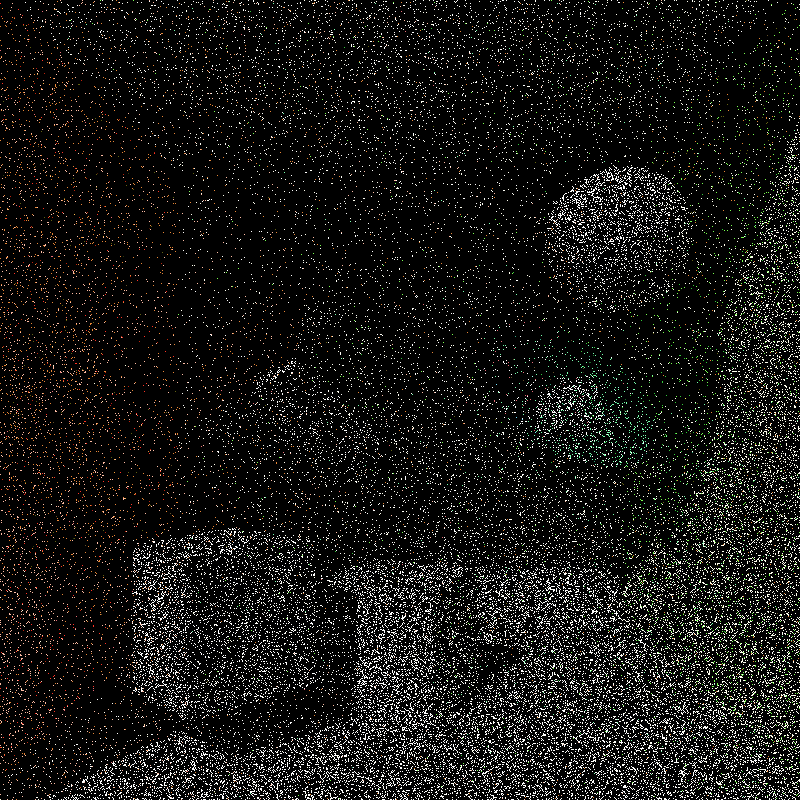
\includegraphics[scale=0.3]{indirect5120.png}
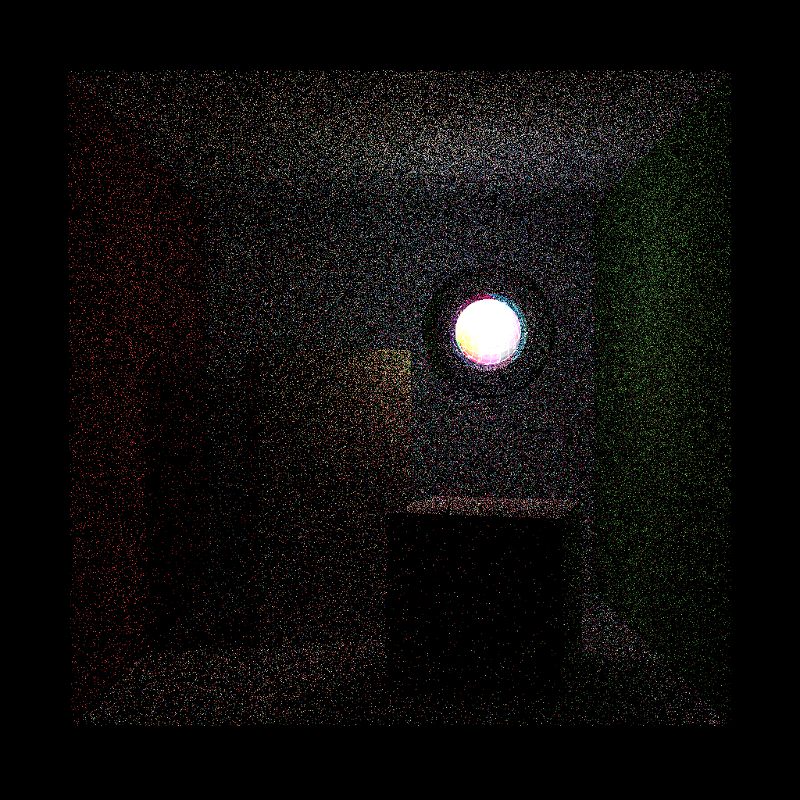
\includegraphics[scale=0.3]{spherelight_16.png}
\caption*{Рисунок 1 --- Шум на изображениях, полученных трассировкой путей}
\end{figure}

Производительность алгоритма трассировки путей может быть многократно увеличена при помощи использования техник понижения дисперсии, програмных оптимизаций и различных эвристик, некоторые из которых затронуты в последующих главах данной курсовой работы.

Из главного преимущества алгоритма трассировки лучей --- универсальности --- следует и его главный недостаток: решение уравнения \eqref{eq:pt} подразумевает фиксацию позиции наблюдателя и, следовательно, представляет собой неподвижное изображение. Теоретически, алгоритм возможно адаптировать для расчета значений в вершинах сцены, заданной полигональной сеткой, однако практика показывает, что такой подход крайне неэффективен.

Для сцен с диффузными поверхностями, т.е. таких, где все ДФОС во всех точках имеет вид $f_r(x) = \dfrac{\rho}{\pi}$, алгоритм трассировки путей также работает крайне неэффективно по той причине, что для расчета излучаемости в таких точках требуется очень большая выборка, которая, из-за рекурсивной природы алгоритма, приводит к запредельным временам расчета для большинства нетривиальных сцен.
\subsection{Метод излучательности}
Помимо алгоритмов, основанных на трассировке лучей, существуют и другие, решающие схожую, но не такую же задачу: расчет освещенности сцены, где каждая точка (поверхность) является рассеивающим отражателем (ДФОС во всех точках равна $\dfrac{\rho}{\pi}$). Для такой сцены уравнение \eqref{eq:kaj} принимает вид
\begin{equation}
L(x) = L_e(x) + \int_{\Omega} f_r(x) L(x \leftarrow \omega_i) \cos(\omega_i, N_x) d \omega_i, \label{eq:diff-kaj}
\end{equation}
то есть не зависит от позиции наблюдателя. В указанных ограничениях возможно получить решение, которое не привязано к одному направленю взгляда и может (по окончанию расчетов) быть использовано для составления интерактивной трехмерной модели.

Одним из таких алгоритмов является \emph{метод излучательности}, основанный на алгоритме расчета теплопередачи и впервые адпатированный для генерации реалистичных изображений в 1984 г. \cite{Gor84}. Основная идея алгоритма заключается в том, что поверхности сцены разбиваются на участки, излучательность на которых полагается константной, и распределение энергии расчитывается между этими участками. Для каждого такого участка входными данными является его собственная излучаемость $B_i^e$ (описывающая его яркость) и отражательная способность $\rho_i$ (в диапозоне от нуля до единицы). За участки часто принимаются полигоны, описывающие сцену, если такая информация доступна.

Следующим шагом решается система линейных уравнений, связывающая излучаемость всех участков сцены. Итогом решения такой системы являются значения $B_i$ для каждого участка, которые затем переводятся в яркость процессом тонального отображения и могут быть отображены на экране с помощью растеризации. Так как вычисленные значения не зависят от позиции наблюдателя, использование графических ускорителей позволяет визуализировать ``освещенную'' сцену в реальном времени с произвольной позиции.
\begin{figure}[h]
\centering
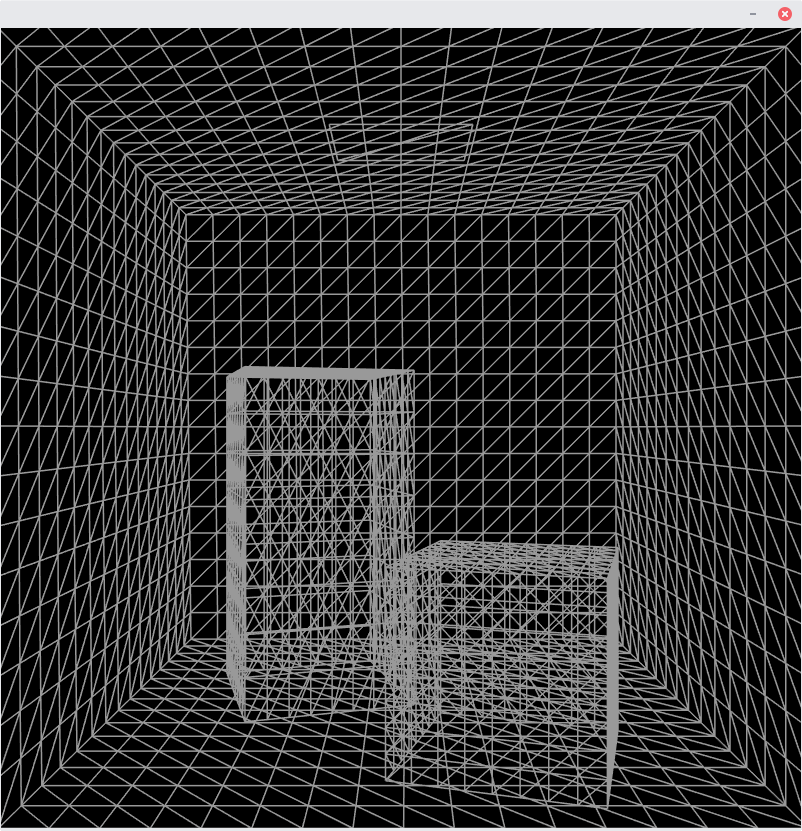
\includegraphics[scale=0.3]{rad_input.png}
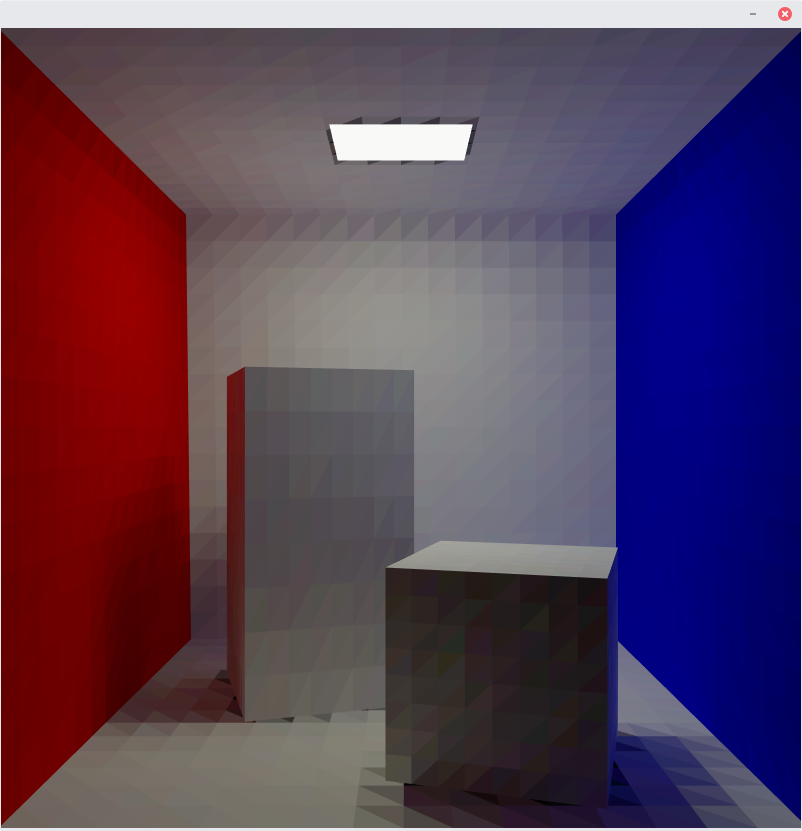
\includegraphics[scale=0.3]{rad_output.png}
\caption*{Рисунок 2 --- Метод излучательности}
\end{figure}

Классический метод излучательности представляет собой частный случай более общего численного метода --- \emph{метода конечных элементов}, широко использующегося в решении задачач гидродинамики, электродинамики и теплообмена. Вкратце, обоснование метода заключается в следующем: из уравнения \eqref{eq:diff-kaj} выводится СЛАУ путем переформулировки интеграла по полушарию на интеграл по всем поверхностям сцены:
\begin{equation}
L(x) = L_e(x) + \rho(x) \int_S K(x, y) L(y) d A_y, \label{eq:kaj-surf}
\end{equation}
ядром интегрирования которой служит функция $K(x,y)$, равная произведению $G(x,y) V(x,y)$, где 
\begin{equation}
G(x,y) = \frac{\cos(\theta_{xy}, N_x) \cos(-\theta_{xy}, N_y)}{\pi r_{xy}^2}\label{eq:geom}
\end{equation}
описывает взаимную ориентацию поверхностей в пространстве, а $V(x,y)$ равняется 1, если точки $x$ и $y$ взаимно видимы, и нулю в противном случае. Затем, полученное равенство используется для выражения средней излучаемости $B_i$ произвольной поверхности, после чего излучаемость полагается константой на каждом выделенном участке, и интеграл переписывается как сумма \cite{Coh93}:
\begin{equation}
\begin{split}
&B_i = B_{ei} + \rho_i \sum_j F_{ij} B_j\\
&F_{ij} = \frac{1}{A_i} \int_{S_i} \int_{S_j} K(x,y) dA_y dA_x, \label{eq:rad}
\end{split}
\end{equation}
систему которых (для всех $i$) называют \emph{системой уравнений метода излучательности}. Коэффициенты $F_{ij}$ обычно называют \emph{форм-факторами}: их вычисление и хранение служат причиной большинства проблем, связанных с реализацией метода. Коль скоро коэффициенты системы расчитаны, остается лишь найти решение получившейся СЛАУ.

Следующая глава данной курсовой работы посвящена описанию и анализу классического метода излучательности, проблем, сопровождающих реализацию оного, и представлению различных модификаций, решающих эти проблемы.
\newpage\section{Разработка алгоритма}
\subsection{Стандартный метод излучательности}
Концептуально, классический метод излучательности состоит из следующих шагов:
\begin{enumerate}
\item разбиение входных данных на участки, излучаемость на которых полагается константной (для данной длины волны);
\item расчет форм-факторов $F_{ij}$ для всех пар $(i, j)$ участков получившейся сцены;
\item численное решение системы уравнений \eqref{eq:rad};
\item отображение решения (включает в себя как процесс тонального отображения, так и преобразование спектральных данных в требуемое цветовое пространство).
\end{enumerate}

Каждый из приведенных шагов может быть реализован с использованием различных методов, выбор которых определяет не только время работы алгоритма, но и количество необходимых для его работы ресурсов: так, форм-факторы могут быть рассчитаны заранее и сохранены в памяти для дальнейшего использования, а могут рассчитываться заново по необходимости.

Последний, четвертый, шаг алгоритма представляет меньше трудностей нежели остальные: физический смысл происходящего прост и понятен, а реализация сводится к выбору оператора тональной компресии, описанному в главе 3.5. Первым же трем шагам сопутствуют трудности, преодоление некоторых из которых как минимум нетривиально. Далее будут описаны проблемы, сопровождающие реализацию метода излучательности в том виде, в котором он представлен в начале настоящей главы.

На первый взгляд это может показаться неочевидным, но даже реализация первого этапа алгоритма вызывает трудности. Для достижения реалистичного результата участки, на которые разбивается сцена, должны быть достаточно небольшими, чтобы передавать все детали освещения (например, на границе резких теней), однако излишнее измельчение сцены приведет к неадекватным временным затратам и требованиям к доступной памяти. В идеале процесс дискретизации сцены должен гарантировать с заданной точностью, что на каждом полученном участке излучаемость будет постоянной.

Больше всего проблем, бесспорно, связано со вторым этапом алгоритма: расчетом и хранением форм-факторов. Во-первых, форм-фактор представляет собой двойной интеграл по поверхности, т.е. для получения искомого значения необходимо решить дифференциальное уравнение четвертой степени, которое  ``даже самого терпеливого преисполнит отвращения и неизбежно оттолкнет от решения задачи'' \cite{Sch93}. Более того, аналитически решение возможно получить только в частом случае взаимно видимых поверхностей, практически не встречающемся в задаче генерации реалистичных изображений. В остальных же случаях интеграл вычислим лишь численными методами, так или иначе включающими в себя многократную проверку взаимной видимости двух произвольных точек сцены. Не облегчает ситуации и тот факт, что подынтегральная функция может иметь разрывы разных степеней, и $r_{xy}^2$ в знаменателе может стремиться к нулю для двух смежных участков. Однако самой серьезной проблемой для любых нетривиальных сцен всегда является количество вычисляемых форм-факторов: в более сложных моделях количество полигонов может исчисляться миллионами, а количество вычисляемых форм-факторов, следовательно, --- триллионами, что далеко выходит за рамки возможностей современных домашних ПК. Вместе с тем, как замечено ранее, недостаточная гранулярность разбиения приводит к потерям деталей и нарушению реализма:
\begin{figure}[h]
\centering
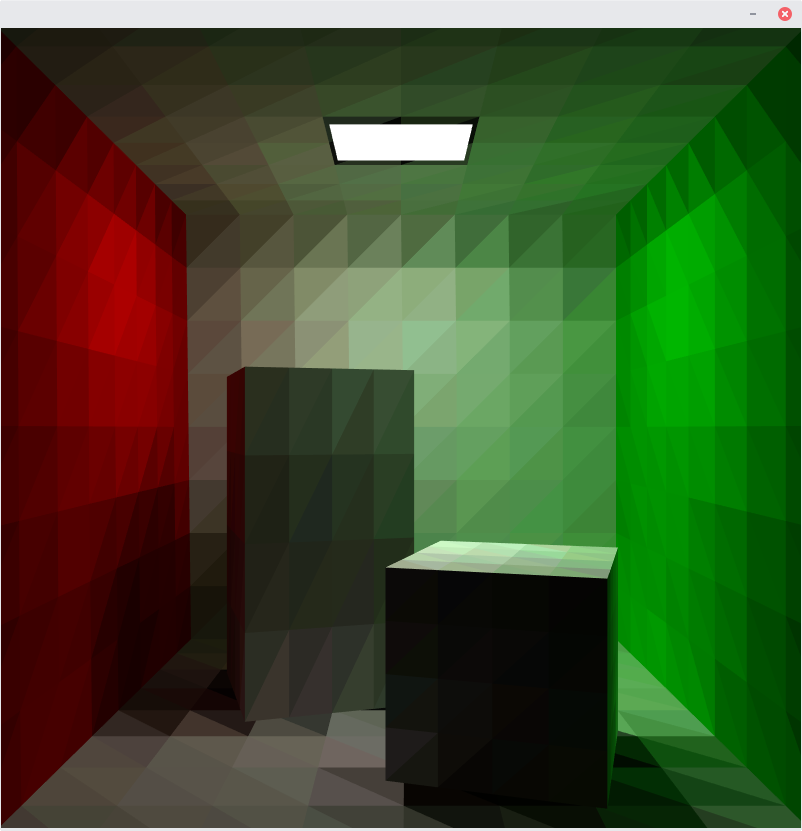
\includegraphics[scale=0.3]{rad_bad1.png}
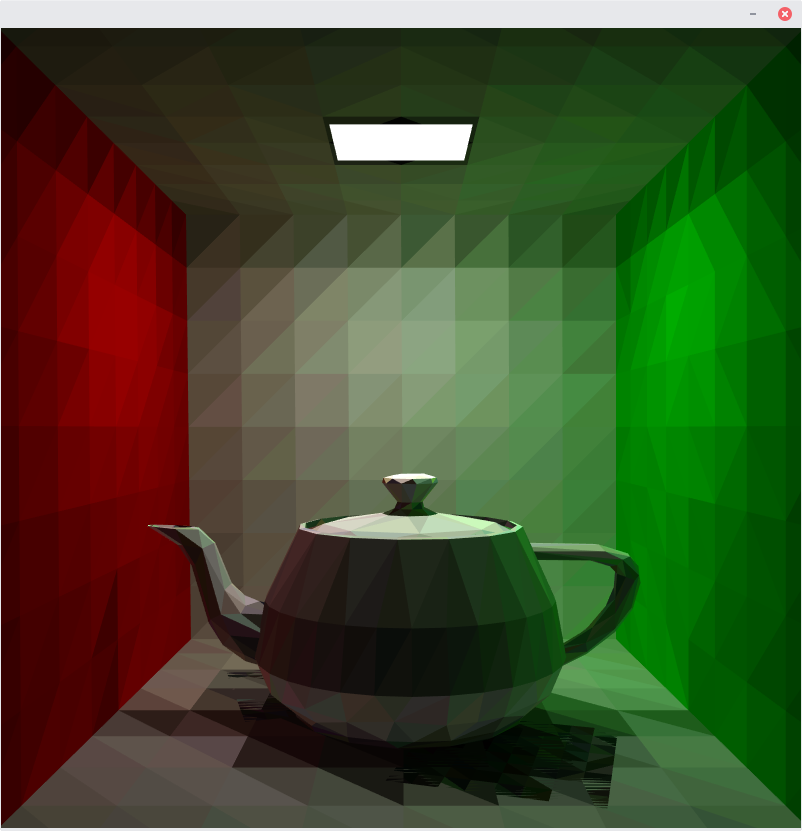
\includegraphics[scale=0.3]{rad_bad2.png}
\caption*{Рисунок 3 --- Артефакты при недостаточном разбиении}
\end{figure}

Решение системы уравнений излучательности \eqref{eq:rad} сложной сцены прямыми методами также нецелесообразно из-за необходимости хранения форм-факторов.
\subsection{Итеративный подход}
Заметим, что матрица коэффициентов системы уравнений излучательности обладает свойством диагонального преобладания \cite{Pet06}, что позволяет использовать итеративный метод Якоби для получения решения с достаточной точностью. Использование итеративного подхода допускает расчет только одной строки форм-факторов в любой момент времени, так как в процессе итерации уточненные значения рассчитываются для каждого участка независимо. Таким образом, проблема хранения квадратичного числа форм-факторов решается в корню. Более того, каждая такая итерация отвечает одному отражению всех световых лучей сцены, что интуитивно понятнее, чем расчет ``всех'' отражений для каждого луча по очереди, и позволяет тривиально организовать процесс предпросмотра получаемого решения.

Более конкретно, итеративный процесс Якоби применим к решению СЛАУ излучательности следующим образом: начальными значениями излучаемости для каждого участка полагается их собственная излучаемость (положительная для источников света и ноль для остальных). Далее, значения последовательно уточняются с использованием приближений, полученных на предыдущей итерации. Приминительно к системе \eqref{eq:rad} использование итеративного метода Якоби дает для каждого участка $i$ следующее выражение:
\begin{equation}
\begin{split}
B_i^{(0)} &= B_{ei}\\
B_i^{(k + 1)} &= B_{ei} + \rho_i \sum_j F_{ij} B_j^{(k)}.\label{eq:iter}
\end{split}
\end{equation}
С использованием метода полукуба \cite{Coh85}, позволяющим получить сразу всю строку форм-факторов для данного участка, становится возможной генерация следующего изображения \cite{Coh85}:
\begin{figure}[h]
\centering
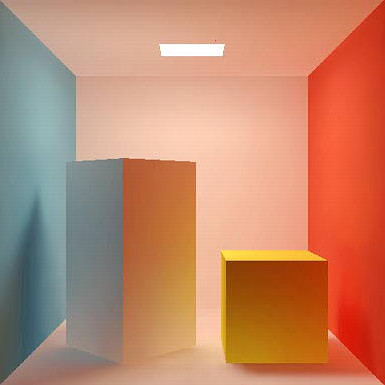
\includegraphics[scale=0.647]{cohen.jpg}
\caption*{Рисунок 4 --- Решение СЛАУ излучательности итеративным методом Якоби}
\end{figure}

Как было сказано, применение итераций Якоби для решения системы уравнений излучательности позволяет не только избавиться от необходимости хранения всех пар форм-факторов в явном виде, но и предоставляет интуитивно понятный процесс получения последовательных приближений. Так, для расчета локальной модели освещения достаточно остановить итеративный процесс после первого же приближения (см. рис. 5).

Однако, хоть проблема хранения и решается описанным методом, сохраняет свою актуальность вопрос вычисления форм-факторов: для получения одного приближения необходимо произвести квадратично зависимое от $N$ число вычислений: $N \cdot (N - 1)~/~2$ двойных интегралов по поверхностям. Сверх того, отказ от хранения форм-факторов приводит к тому, что на кажой итерации значения рассчитываются заново! Из этого следует, в том числе, что при недостаточно точно вычисляемых значениях форм-факторов, используемые итерации могут вообще не дать годного к использованию решения за адекватное время.

В следующей главе представлен т.н. \emph{метод локальных линий}, в котором форм-факторы рассматриваются как вероятности, и потому могут быть приближены с использованием статистических методов и, что самое главное, вычисляться неявно, в следствие чего проблемы хранения и повторного вычисления форм-факторов попросту исчезают. 

\begin{figure}[h]
\centering
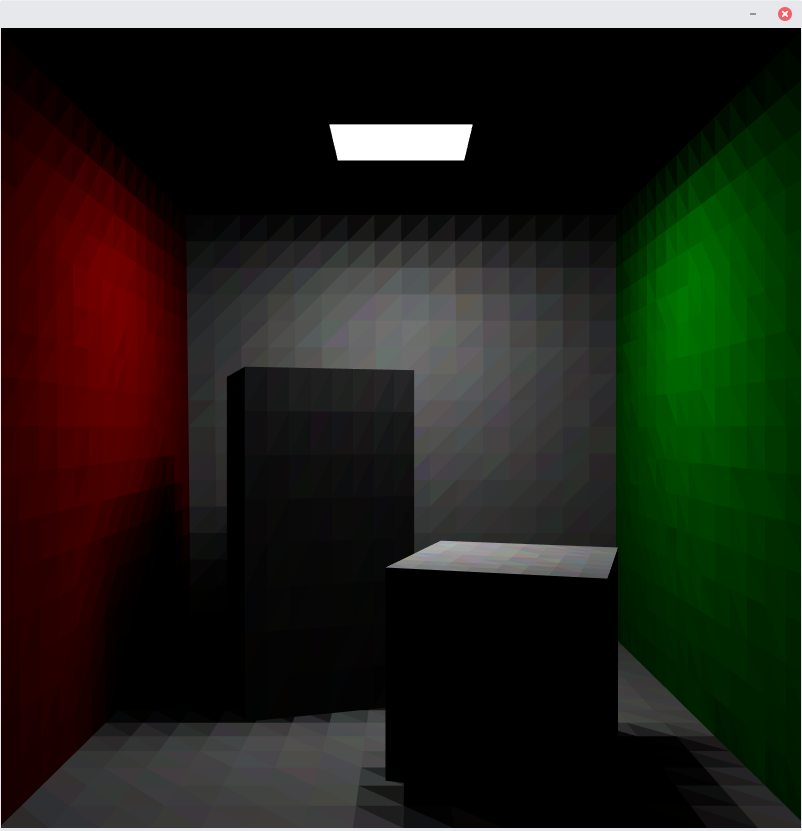
\includegraphics[scale=0.3]{direct_only.png}
\caption*{Рисунок 5 --- Результат работы одной итерации алгоритма}
\end{figure}

\subsection{Метод локальных линий}
Рассмотрим формулу для форм-факторов из уравнения \eqref{eq:rad}: значение подынтегральной функции, а значит и самого интеграла, всегда принимает неотрицательные значения. Взглянем теперь на сумму всех форм-факторов $F_{ij}$ для фиксированного участка $i$:
\begin{equation}
\begin{split}
\sum_j F_{ij} &= \frac{1}{A_i} \int_{S_i} \sum_j \int_{S_j} K(x,y) dA_y dA_x = \\
&= \frac{1}{A_i} \int_S K(x,y) dA_y dA_x.
\label{eq:ff-sum}
\end{split}
\end{equation}
Переформулировав интеграл обратно в термины направлений, получим
\begin{equation}
\begin{split}
\sum_j F_{ij} &= \frac{1}{A_i} \int_{S_i} \frac{1}{\pi} \int_{\Omega_x} \cos(\theta_{xy}, N_x) d\theta_{xy} dA_x\\
&= \frac{1}{A_i} \int_{S_i} \frac{\pi}{\pi} dA_x= 1.
\label{eq:ff-sum2}
\end{split}
\end{equation}
Таким образом, сумма всех форм-факторов для данного участка равняется единице (в случае незамкнутой сцены сумма может принимать меньшие значения). Наконец заметим, что простая перестановка порядка интегралов позволяет убедиться, что для любых $i$, $j$
\begin{equation}
A_i F_{ij} = A_j F_{ji}.\label{eq:ff-rep}
\end{equation}
Перечисленный набор свойств позволяет рассматривать форм-факторы $F_{ij}$ как набор \emph{вероятностей}. Вспомним теперь, что (за вычетом собственной излучаемости) форм-фактор $F_{ij}$ описывает \emph{долю} излучаемости участка $i$, происходящюю от участка $j$. Учитывая, что энергия $P_i$ и излучаемость $B_i$ данного участка различаются лишь зависимостью от площади: $P_i = A_i B_i$, систему уравнений излучательности можно переформулировать с использованием энергии:
\begin{equation}
P_i = P_{ei} + \sum_j P_j F_{ji} \rho_i, \label{eq:rad-pow}
\end{equation}
где $F_{ji}$ обозначает часть энергии участка $i$ (за вычетом излучаемой), отвечающей участку $j$, или, что то же самое, $F_{ij}$ обозначает часть энергии участка $i$ (за вычетом излучаемой), попадающей на участок $j$. Такая формулировка позволяет получить приблизительное значение форм-факторов $F_{ij}$ для участка $i$ при помощи простейшей симуляции, выпустив $N_i$ лучей из случайных точек участка и распределенных согласно закону косинусов в полушаре вокруг нормали. Тогда отношение $N_j / N_i$ попавших в участок $j$ лучей к общему их числу будет приблизительно равно форм-фактору $F_{ij}$ \cite{Shir90}.
\begin{figure}[h]
\centering
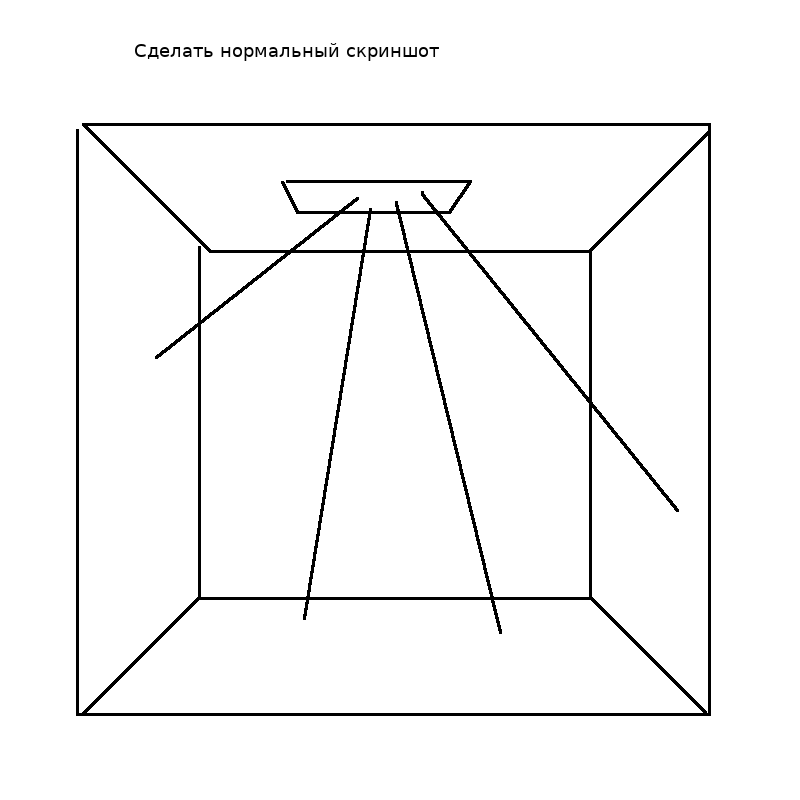
\includegraphics[scale=0.3]{local_lines.png}
\caption*{Рисунок 6 --- Расчет форм-факторов с использованием локальных линий}
\end{figure}

Описанный процесс симуляции не должен использоваться непосредственно, так как до сих пор подразумевает явный расчет значений форм-факторов. Ценность подхода заключается в переформулировке проблемы подсчета искомых значений: выражение форм-фактора в качестве суммы позволяет (с учетом описанных выше свойтв) применить к вычислению этой суммы метод Монте-Карло, чему и посвящена следующая глава настоящей работы.

\subsection{Стохастический алгоритм}
Проведя дальнейший анализ, можно получить формулировку теоремы 5.1. из \cite{Bek99}, утверждающую, что ``форм-фактор $F_{ij}$ между двумя участками $i$ и $j$ в дисретизированной сцене соотвествует вероятности $p_{ij}$ того, что случайно выбранный в соответствии с равномерным распределением луч с началом в случайной точке участка $i$ первым пересечет участок $j$ данной сцены''. Для вычисления одного значения форм-фактора данное утверждение никак не упрощает решение поставленной задачи, однако для расчета значений \emph{всех} форм-факторов для фиксорованного участка $i$, описанная процедура может использоваться без изменений! Точнее, используемая в алгоритме статистическая оценка может без дополнительных модификаций быть применена для расчета всей строки форм-факторов одновременно: попадание в любой участок $j$ уточняет значение форм-фактора $F_{ij}$, вне зависимости от $j$. 

С учетом сказанного выше, для расчета всех форм-факторов фиксированного участка $i$ достаточно следующей процедуры \cite{Bek99}:
\begin{framed}
\begin{enumerate}
\item инициализировать все $F_{ij} = 0$
\item для всех $k = 1, \ldots, N$
\begin{enumerate}
    \item[(а)] выбрать случайную точку $x$ на участке $i$
    \item[(б)] выбрать случайное направление $\Theta_x$ из полушара вокруг нормали к участку $i$ в точке $x$ в соотвествии с распределением косинусов
    \item[(в)] найти ближайшее пересечение построенного луча с поверхностью $j$ сцены, запомнить $j$
    \item[(г)] $F_{ij} = F_{ij} + \dfrac{1}{N}$ 
\end{enumerate}
\end{enumerate}
\end{framed}
\begin{center}Листинг 1 --- Расчет строки форм-факторов методом Монте-Карло\end{center}

где $N$ означает количество лучей, выпускаемых из участка $i$, и правильный выбор $N$ позволяет избавиться от необходимости явного вычисления и, как следствие, хранения форм-факторов.

Переформулировав итерации Якоби \eqref{eq:iter} с терминов энергии \eqref{eq:rad-pow} на термины \emph{нераспределенной} энергии:
\begin{equation}
\Delta P_i^{(k+1)} = \sum_{j \neq i} \Delta P_j^{(k)} F_{ji} \rho_i, \label{eq:rad-pow-d}
\end{equation}

приняв вероятность выбора участка $i$ за $p_i = \Delta P_j^{(k)} / \Delta P_T^{(k)} = \sum\limits_i \Delta P_i^{(k)}$ и  использовав районированную выборку по значимости (анлг: stratified importance sampling), можно получить итоговый алгоритм \cite{Bek99}, назыаемый \emph{инкрементанльным стохастическим итеративным методом Якоби (англ: incremental stochastic Jacobi iterative method)}. В дополнение к сказанному, для удобства реализации можно ввести для каждого участка значения $\delta P_i$, обозначающие полученную на данной итерации энергию. По окончанию итерации, нераспределенная энергия полагается равной полученной, а полученная обнуляется:
\begin{framed}
\begin{enumerate}
\item инициализировать общую энергию $P_i = B_{ei} \cdot A_i$, нераспределенную энергию $\Delta P_i = B_{ei} \cdot A_i$, полученную энергию $\delta P_i = 0$ для всех участков $i$, и вычислить общую нераспределенную энергию $\Delta P_T = \sum\limits_i \delta P_i$
\item продолжать пока для $||\Delta P_i|| \leqslant \varepsilon$ или не будет превышено маскимальное количество итераций:
\begin{enumerate}
    \item[(а)] выбрать количество лучей $N$
    \item[(б)] сгенерировать случайное число $\xi \in (0, 1)$
    \item[(в)] инициализировать $N_{\text{prev}} = 0$, $q = 0$
    \item[(г)] для каждого участка $i$:
    \begin{enumerate}
        \item[i.] $q_i = \Delta P_i / \Delta P_T$
        \item[ii.] $q = q + q_i$
        \item[iii.] $N_i = \lfloor Nq + \xi \rfloor - N_{\text{prev}}$
        \item[iv.] повторить $N_i$ раз:
        \begin{enumerate}
            \item[А.] выбрать случайную точку $x$ на участке $i$
            \item[Б.] выбрать случайное (согласно описанному распределению) направление $\Theta$ из точки $x$
            \item[В.] определить участок $j$, содержащий первое пересечение луча с началом в $x$ в направлении $\Theta$ с поверхностями сцены
            \item[Г.] увеличить $\delta P_j = \delta P_j + \dfrac{1}{N} \rho_j \Delta P_T$
        \end{enumerate}
        \item[v.] $N_{\text{prev}} = N_{\text{prev}} + N_i$
    \end{enumerate}
    \item[(д)] пройтись по всем участкам $i$, увеличить энергию $P_i = P_i + \delta P_i$, заменить нераспределенную энергию $\Delta P_i = \delta P_i$ и обнулить полученную энергию $\delta P_i$. На лету пересчитать общие для сцены величины $P_T$ и $\Delta P_T$
    \item[(е)] отобразить полученный результат с использованием $P_i$.
\end{enumerate}
\end{enumerate}
\end{framed}
\begin{center}
Листинг 2 --- Инкрементанльный стохастический итеративный метод Якоби 
\end{center}

В приведенном виде алгоритм всё же не может использоваться для получения цветных изображений: описанную процедуру необходимо проводить спектрально, для каждой длины волны. Более того, так как алгоритм опирается на нахождение пересечений с объектами сцены, необходимо эффективно организвать доступ к геометрии сцены, иначе с ростом детализации время работы алгоритма будет расти с квадратичной завимостью от оной.

Для относительно простой же сцены, с проведением трех независимых симуляций для красного, синего и зеленого цветов, описанный метод позволяет получить следующие изображения:
\begin{figure}[h]
\centering
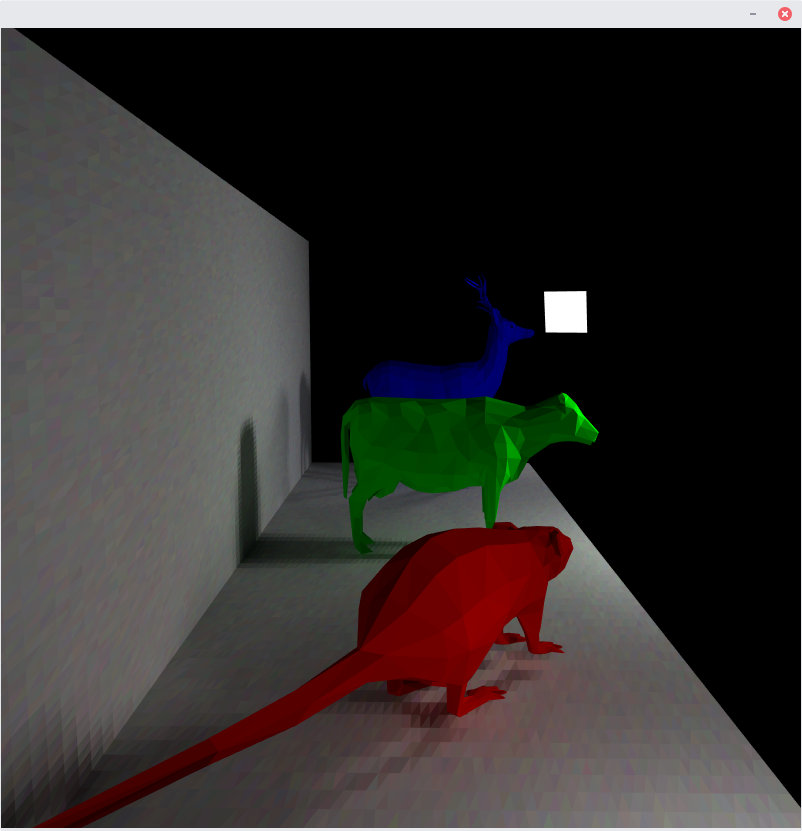
\includegraphics[scale=0.3]{photoshoot_1.png}
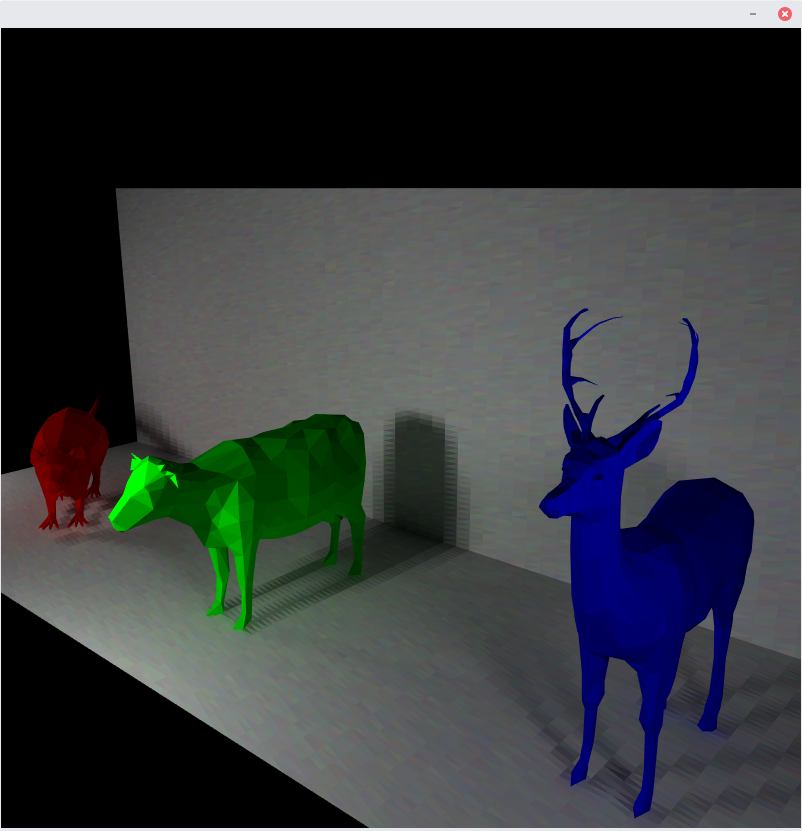
\includegraphics[scale=0.3]{photoshoot_2.png}
\caption*{Рисунок 7 --- Результат работы ИСИМЯ для трех длин волн}
\end{figure}
\subsection{Модификации и ускорения}
С применением простейших модификаций, описанных выше, алгоритм работает корректно, и может быть использован для получения изображений. Однако специфика выбранных методик открывает огромный простор для различных модификаций и ускорений. Так, расчет сумм методом Монте-Карло позволяет использовать широкий набор методов для понижения дисперсии: выборка по значимости и районированная выборка уже включены в листинг 2; использование для генерации точек и направлений последовательностей с низкой расходимостью (англ: low-discrepancy sequence) позволяет в некоторых случаях получить ускорение вплоть до одного порядка \cite{Kel96}; существенно ускорить сходимость можно при помощи использования метода выделения главной части (англ: control variates); лучший результат дает также множественная выборка по значимости (анлг: multiple importance sampling).

Помимо техник уменьшения вариации, возможно адаптировать алгоритм для параллельных вычислений: расчеты могут производиться  для нескольких участков одновременно, с незначительным количеством обращений к разделяемым ресурсам и затранам на синхронизацию. Выбор и реализация структуры хранения сцены же в целом играют ключевую роль в быстродействии всей программы. 
\newpage\section{Реализация}
Для реализации описанного в главе 2 алгоритма было написано приложение, осуществляющее загрузку и обработку полигональной модели в формате wavefront obj и построение эффективного представления сцены в виде BVH-дерева с тем, чтобы ускорить все необходимые для расчетов операции. По окончанию работы алгоритма производится приведение полученных значений излучаемости к формату RGB для последующего их отображения на экране.

Языком реализации был выбран C++11. Для отображения промежуточных и конечных результатов и организации взаимодейтвия с пользователем использовались OpenGL API и библиотека GLFW соответственно.
\subsection{Общая структура приложения}
Файлы приложения были разбиты на каталоги: 
\begin{enumerate}
\item[] \texttt{includes/} --- для хранения заголовочных файлов и файла констант;
\item[] \texttt{src/} --- для хранения исходного кода;
\item[] \texttt{models/} -- для хранения полигональных моделей и данных о материалах;
\item[] \texttt{glsl/} --- для хранения используемых шейдеров
\end{enumerate}

Для сборки приложения был написан простейший Makefile:
\begin{lstlisting}[language=Bash]
APP_NAME=rad
APP_SRCS=src/*.cpp
CFLAGS=-g -O2 -lGLEW -lglfw -lGL -pthread
CC=g++

all: $(SERVER_SRCS)
	$(CC) -o $(APP_NAME) $(APP_SRCS) $(CFLAGS)

clean:
	/bin/rm -f rad
\end{lstlisting}
\begin{center}Листинг 3 --- Файл сборки проекта\end{center}

Работу программы можно условно разбить на следующие блоки: инициализация OpenGL, загрузка констант, настройка необходимых для работы параметров OpenGL, загрузка полигональной модели, запуск основного цилка отображения и (параллельно с предыдущим) алгоритма излучательности.

Из соображений обратной совместимости для реализации приложения использовалась версия 3.3 OpenGL API. Так как расчеты излучательности целиком производились на центральном процессоре, для сглаживания изображения возможно стало использовать мультисэмплинг (анлг: multisample anti-aliasing, MSAA). 

Так как с ростом числа файлов в проекте время компиляции стало превышать 10-15 секунд (что в некоторых случаях сравнимо со временем работы алгоритма), большинство параметризованных величин было вынесено в файл \texttt{includes/constants}, который загружается при каждом запуске программы, таким образом освобождая пользователя от необходимости повторно компилировать приложение при изменении каких-либо констант.

Для отображения данных на экране был написан простейший шейдер, принимающий значения позиции и цвета и прямо передающий их на отрисовку:
\begin{lstlisting}
#version 330 core

layout (location = 0) in vec3 position;
layout (location = 1) in vec3 color;

uniform mat4 proj;
uniform mat4 view;

out vec3 fragColor;

void main() {
    fragColor = color;
    gl_Position = proj * view * vec4(position, 1.0f);
}
\end{lstlisting}
\begin{center}Листинг 4 --- Вершинный шейдер\end{center}

С целью упрощения процесса использования шейдеров был написан класс \texttt{utils::shader}, предоставляющий интуитивные методы для создания и использования шейдерной программы и установки значений ``единых переменных'' (англ: uniform variables). Так как OpenGL API предлагает использовать различные функции для установки значений единых переменных различных типов, для шаблона метода \texttt{utils::shader::set\_uniform<T>} были написаны специализации со всеми поддерживаемыми типами. Не вдаваясь в подробности, использование класса упрощается до подключения заголовочного файла \texttt{includes/shader.h} и последующего вызова описанных методов:
\begin{lstlisting}
...
utils::shader shader("glsl/pass_3d.vert", "glsl/white.frag");
shader.use_program();
shader.set_uniform<glm::mat4>("proj", proj);
shader.set_uniform<glm::mat4>("view", view);
...
\end{lstlisting}
\begin{center}Листинг 5 --- Использование класса шейдера\end{center}

Для организации взаимодействия с пользователем была задействована библиотека GLFW и написан класс \texttt{utils::camera}, представляющий собой по сути один метод \texttt{view\_matrix()}, возвращающий видовую матрицу, основываясь на начальных и текущих данных о положении и ориентации камеры. Два простейших коллбэка на каждой итерации основного цикла GLFW актуализируют информацию в классе камеры, опираясь на данные о вводе с клавиатуры и мыши. Для удобства пользования был также введен переключатель между интерактивным режимом и режимом просмотра: в интерактивном режиме передвижения курсора используются для изменения ориентации, а клавиатура --- для изменения положения камеры. В режиме просмотра же движения мыши игнорируются, и обрабатывается только два нажатия клавиатуры: переход обратно в интерактивный режим и выход из приложения.

Наконец, функция, реализующая метод излучательности и тонального отображения, вызывается в отдельном потоке. Таким образом, основной цикл GLFW никогда не останавивается, и процесс ввода работает корректно на протяжении всего жизненного цикла приложения:
\begin{lstlisting}
/* Radiosity and tone-mapping thread */
std::thread t1(radiate,
               std::ref(patches),
               std::ref(primitives),
               std::ref(vertices),
               &tree, s);

/* Main draw loop */
while (glfwWindowShouldClose(window) == 0) {
    ...
    glfwSwapBuffers(window);
}
t1.join();
\end{lstlisting}
\begin{center}Листинг 6 --- Запуск расчетов в отдельном потоке\end{center}

\subsection{Загрузка полигональной модели}
Участками константной излучательности были положены сами полигоны сцены, поэтому процесс предобработки сцены упростился до загрузки полигональной модели и создания массива структур \texttt{patch}, обладающих набором всех необходимых для работы программы полей:
\begin{lstlisting}
struct patch {
    glm::vec3 vertices[4], colors[4];
    glm::vec3 normal, color, emit, p_total, p_unshot, p_recieved;
    float area;
};
\end{lstlisting}
\begin{center}Листинг 7 --- Структура, содержащая данные об участке дискретизации \end{center}

Для загрузки данных из wavefront obj файла был использован заголовочный файл-библиотека\\ \texttt{tinyobjloader.h} \cite{Fuj12}, позволяющий последовательно получить информацию о всех полигонах сцены. Первые три поля массива \texttt{vertices} заполнялись данными из файла, в четвертое же записывался центроид, а в поле \texttt{area} --- площадь полученного треугольника. Поля \texttt{normal}, \texttt{color} и \texttt{emit} также заполнялись без каких-либо дополнительных модификаций.
\subsection{Построение BVH-дерева}
Так как предложенный в главе 2 алгоритм опирается на возможность определить первое пересечение произвольного луча со сценой, для эффективной реализации необходимо составить структуру данных, позволяющую за минимальное время найти такое пересечение. В качестве такой структуры было выбрано BVH-дерево (англ: bounding volume hierarchy, BVH) \cite{KK86}. Кратко, эта структура представляет из себя дерево, корнем которого является минимальный параллелепипед с ребрами, параллельными осям координат (анлг: axis-aligned bounding box, AABB), содержащий центроиды всех объектов сцены. Если узел такого дерева не является листом, то в нем содержится два указателя на устроенные аналогично дочерние узлы. Каждый из дочерних элементов содержит подмножество элементов своего родителя, причем множества элементов узлов с одинаковым родителем не пересекаются.  Болеее того, каждый примитив, содержащийся в дереве, встречается во всей иерархии только один раз. 

В рамках данной курсовой работы использовалась упрощенная реализация BVH-дерева из \cite{Pha17}: построение структуры разбивается на два этапа: нахождение AABB для каждого примитива сцены, и построение иерархии на основе одного из выбранных алгоритмов разбиения. С целью повышения эффективности, алгоритм принимает на вход вектор указателей на структуры \texttt{patch}. Вся же необходимая информация о данном примитиве хранится в справочном векторе структур \texttt{prim\_info}:
\begin{lstlisting}
struct prim_info {
    std::size_t prim_idx;
    aabb box;
    glm::vec3 centroid;
};
\end{lstlisting}
\begin{center}Листинг 8 --- Структура, содержащая данные о примитиве \end{center}

Так, первый этап построения дерева заключается в проходе по всем примитивам, расчету для каждого из них максимальной и минимальной координат $x$, $y$ и $z$ и записи их в справочную структуру по соответсвующему индексу.

Далее, вызывается рекурсивная процедура \texttt{rec\_build}, инициализирующая и возвращающая узел дерева. Вне зависимости от количества количества переданных примитивов первым шагом процедура вычисляет объединение всех актуальных AABB с использованием функции \texttt{join}, находящей ``AABB двух AABB''. Затем, в зависимости от количества переданных примитивов (на самом деле в функцию передаются не примитивы, а лишь их количество и индекс первого примитива в массиве указателей), либо возвращаемый узел инициализируется в лист, либо вызывается функция деления примитивов. Выбор этой функции является определяющим как с точки зрения сложности реализации, так и в быстродействии получившейся структуры. Так как в задачи данной курсовой работы не входит изучение тонкостей построения деревьев двоичного разбиения пространства, для деления примитивов была выбрана простейшая функция разбиения на подмножества равного размера: после выбора оси разбиения вызывается функция \texttt{std::nth\_element}, принимающая серединный элемент и функцию сравнения и за линейное время приводящая массив в такое состояние, что все элементы, меньшие серединного оказываются перед оным, а большие --- после. Реализация, предложенная в \cite{Pha17}, также включает в себя вектор \texttt{ordered\_primitives}, в который в ходе построения дерева последовательно добавляются указатели на примитивы в том порядке, в котором это необходимо для последующего использования алгоритма; по окончанию работы рекурсивной процедуры этот вектор обменивается с переданным в функцию:
\begin{lstlisting}
bvh_node *bvh(std::vector<patch *> &primitives) {
    std::vector<prim_info> primitive_info(primitives.size());
    std::vector<patch *> ordered_primititves;

    /* Bounding volumes for each primitive */
    for (std::size_t i = 0; i < primitives.size(); i++) {
        auto box = compute_box({*primitives[i]});
        primitive_info[i] = {i, box, (box.near + box.far) / 2.0f};
    }

    /* Construct the BVH */
    bvh_node *root = rec_build(primitive_info, 0, primitives.size(), 
                               ordered_primititves, primitives);
    std::swap(ordered_primititves, primitives);

    return root;
}
\end{lstlisting}
\begin{center}Листинг 9 --- Построение BVH-дерева \end{center}

Последующее использование полученного дерева опирается на тот факт, что если луч не пересекается с AABB группы примитивов, то он точно не пересекает ни один из этих примитивов. Таким образом, для рассчета параметра первого пересечения луча со сценой достаточно простой рекурсивной процедуры, обрабатывающей два случая: если переданный узел является листом, то каждый содержашийся в нем примитив проверяется на пересечение с лучем, и возвращается минимальное значение параметра; в противном же случае процедура вызывается рекурсивно для обоих дочерних элементов, и возвращается минимальное из двух полученных значений. Для целей данной курсовой работы необходимо было получать не только параметр перечения, но и прочую информацию о точке попадания луча, такую как наличие самого факта попадания и данные пересеченного участка, если таковой имеется. Для этого из функции пересечения возвращалась структура \texttt{hit}:
\begin{lstlisting}
struct hit { bool hit; float t; patch *p; };
hit intersect(const ray &r, const bvh_node *node,
              const std::vector<patch *> &primitives, float ERR) {
    if (!intersect(r, node->box, ERR)) { return { false }; }
    hit ret = { false, INF, nullptr };
    if (node->split == axis::none) { ret = ...; } // leaf
    else { // node
        auto hit_c0 = intersect(r, node->children[0], primitives, ERR);
        auto hit_c1 = intersect(r, node->children[1], primitives, ERR);
        if (...) { ... ret = hit_c0; }
        else if (...) { ... ret = hit_c1; }
    }
    return ret;
}
\end{lstlisting}
\begin{center}Листинг 10 --- Пересечение луча с BVH-деревом \end{center}
\subsection{Расчет излучательности}
С учетом сказанного в главе, посвященной разработке алгоритма, реализация инкрементанльного стохастического итеративного метода Якоби упрощается до конкретизации псеводокода, представленного в листинге 2. А именно, до реализации следующих операций: определение общего количества лучей $N$, распространяющих энергию на данной итерации; получение случайной точки в заданном треугольнике и получение случайного направления из полусферы вокруг данной нормали (согласно распределению косинусов).

С целью гарантии того, что каждый выпущенный в ходе симуляции луч будет нести один и тот же квант энергии, число лучей $N$ выбиралось пропорционально объему нераспределенной энергии в сцене \cite{Pet06}: $N = \Delta P^{(k)} / P_T  \cdot N_{\text{total}}$, где общее количество лучей $N_{\text{total}}$ параметризовано и задается при запуске программы в файле констант.

Для получения случайной точки была написана процедура, принимающая три вершины треугольника и использующая два случайных значения из промежутка $[0, 1]$ в качестве барицентрических координат с последующим переходом обратно в декартову систему:
\begin{lstlisting}
/* r1, r2 random from [0, 1]*/
return glm::vec3((1 - glm::sqrt(r1)) * p->vertices[0] 
                 + glm::sqrt(r1) * (1 - r2) * p->vertices[1] 
                 + r2 * glm::sqrt(r1) * p->vertices[2]);
\end{lstlisting}
\begin{center}Листинг 11 --- Генерация случайной точки на треугольнике \end{center}

Направления генерировались в полусферических координатах (с учетом распределения косинусов), а затем переводились в касательное пространство:
\begin{lstlisting}
glm::vec3 sample_hemi(const glm::vec3 &normal) {
    glm::vec3 tan = ... bitan = ...                // tangent, bitangent               
    float u = unilateral(mt), v = unilateral(mt);  // random from (0, 1)
    float cos_theta = glm::sqrt(1 - u);
    float sin_theta = glm::sqrt(1 - cos_theta * cos_theta);
    float phi = 2 * PI * v;
    float x = sin_theta * glm::cos(phi), y = cos_theta, z = sin_theta * glm::sin(phi);
    return glm::normalize(tan * x + normal * y + bitan * z);
}
\end{lstlisting}
\begin{center}Листинг 12 --- Генерация случайного направления из полусферы вокруг нормали \end{center}

Все локальные для каждого участка данные хранились в структуре, описанной в листинге 7. Генерация случайного числа в в диапозоне $(0, 1)$ производилась с использованием класса, предоставляемого стандартной библиотекой С++11: \texttt{std::uniform\_real\_distribution}. Симуляция запускалась три раза: по одному для каждой цветовой составляющей, из-за чего при невысоком количестве лучей на изображениях можно наблюдать RGB-шум:

\begin{figure}[h]
\centering
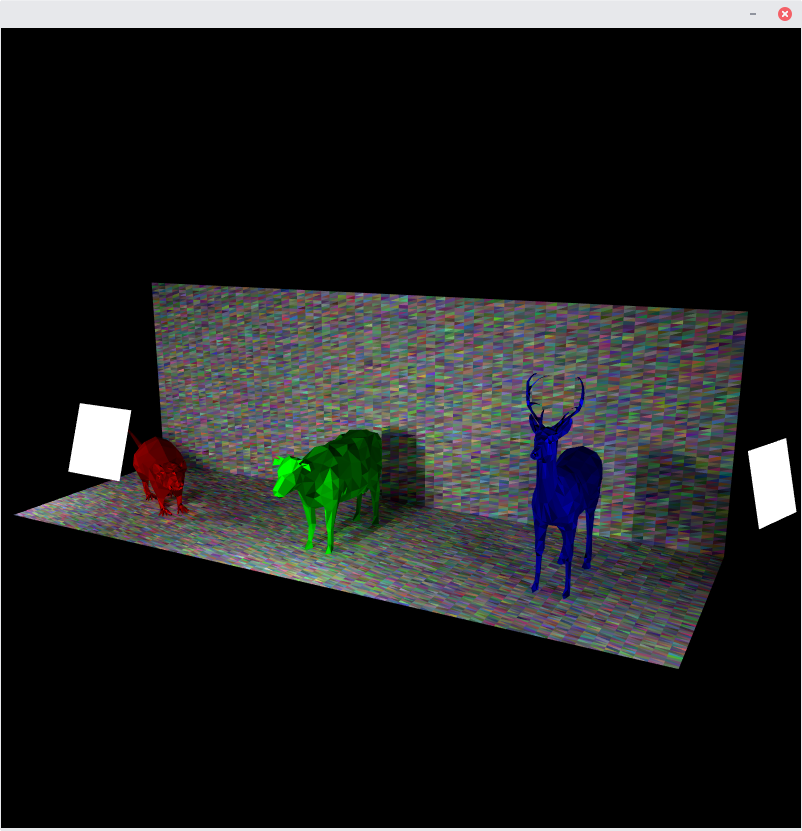
\includegraphics[scale=0.3]{rgb_noise.png}
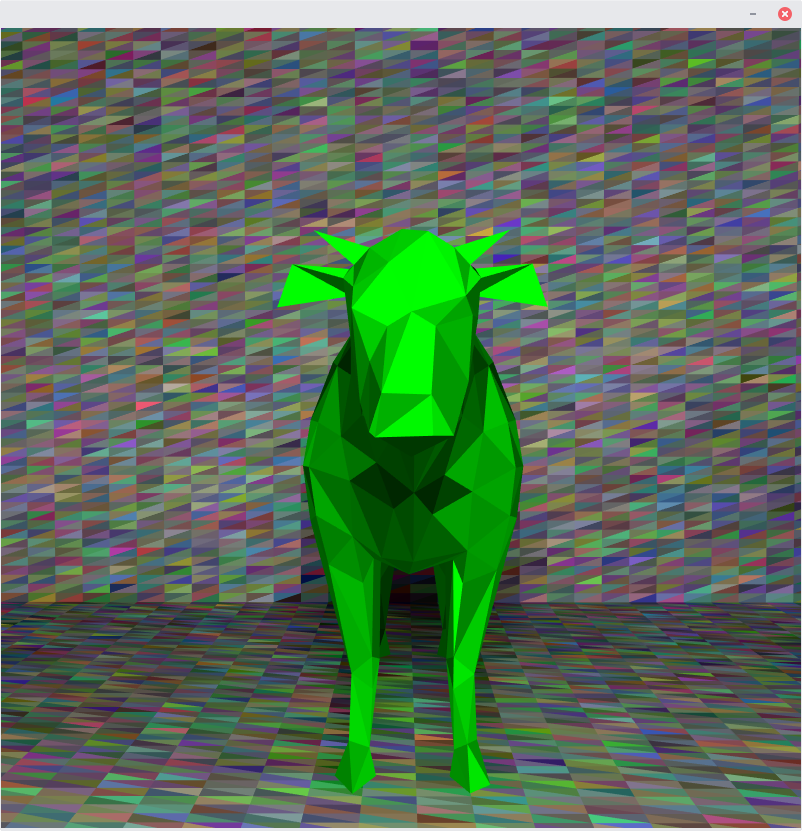
\includegraphics[scale=0.3]{rgb_noise2.png}
\caption*{Рисунок 8 --- Цветовой шум при низком общем количестве лучей}
\end{figure}

\subsection{Тональное отображение}
Вернувшись к поставновке проблемы, решаемой алгоритмами глобального освещения (рассчету значений излучаемости для каждой выбранной единицы дискретизации), можно увидеть, что само по себе такое полученное решение с трудом можно использовать в практических целях. Дело в том, что хоть зрительный аппарат человека и чувствителен к очень большому диапазону излучаемостей (вплоть до 100000000:1), между рассчитанными значениями и зрачком наблюдателя всегда находится некоторый медиум, отображающий полученное решение, будь то один из видов мониторов, проектор, или что-то еще. Динамический диапазон техниики такого вида практически всегда уступает как указанному выше диапазону человеческого зрения, так и встречающимся в реальном мире уровням контрастности (прибл. 80000000:1). Более того, хоть монитор (проектор и т.п.) и производит на выход ``реальные'' физические величины (кандела / кв. м), входные данные всегда ограничены выбранным протоколом коммуникации, а точнее количеством бит, выделенных на передачу уровней яркости одного цвета. Сверх сказанного, линейные изменения переданных входных значений не отвечают линейным изменениям уровня воспринимаемой яркости.

Последняя проблема решается известным приемом, называемым \emph{гамма-коррекцией}, и заключающемся в переносе всех производимых в программе расчетов в линейное цветовое пространство с последующим возвращением посчитанных значений обратно в ожидаемый монитором вид. В случае OpenGL API возможно реализация гамма-коррекции вручную, во фрагментном шейдере. Однако гораздо удобнее использовать встроенную возможность OpenGL, регулирующуюся флагом \texttt{GL\_FRAMEBUFFER\_SRGB}:
\begin{lstlisting}
glEnable(GL_FRAMEBUFFER_SRGB);
\end{lstlisting}
\begin{center}Листинг 13 --- Включение гамма-коррекции в OpenGL API \end{center}

Решение же проблемы умещения ``реального'' диапозона яркостей в предоставленные дискретные уровни требует специального процесса, называемого \emph{тональной компрессией} или \emph{тональным отображением} (англ: tone mapping). Более формально, этот процесс проводится при помощи т.н. оператора тональой компресии, строящего отображение из всех встречающихся в сцене уровней яркости в отрезок $[0; 1]$. Примером простейшего (хоть и некачественного) оператора тональной компресии можно считать деление всех яркостей на максимальную, встречающуюся в сцене. Как несложно догадаться, если в данной сцене встречается хоть один источник света, то все остальные объекты (особенно не освещаемые непосредственно) будут слишком темными. В качестве другого примера можно рассмотреть оператор, осуществляющий ``зажим'' (англ: clamping) всех значений в пределах отрезка $[0; 1]$, т.е. для любого значения, большего единицы, яркость полагается равной единице. Однако и такой метод не дает ничего близкого к преемлемым результатам для произвольных сцен.

В качестве оператора тональной компресии в данной курсовой работе был выбран т.н. оператор Реинхарда \cite{Rei02}, представленный в 2002 г. Точнее, в \cite{Rei02} описывается два варианта оператора: глобальный и локальный. Глобальный вариант подразумевает компрессию тонов, применяемую равномерно ко всему изображению, в том время как локальный вариант оператора использует информацию о яркости окружающих пикселей и потому предоставляет более качественное решение, но более сложен в реализации, нежели глобальный.

Для отображения тонов использовался глобальный вариант оператора Ренихарда, который применялся к яркостям в каждой вершине используемой полигональной модели. Не останавливаясь на проблемах, специфичных для любой программной реализации алгоритма, таких как деление на ноль, машинная точность и т.п., используемый алгоритм имеет следующий вид:
\begin{equation}
\begin{split}
&L_{\text{средн.}} = exp \left( \frac{1}{N} \sum_{x, y} \log \left( L(x,y) \right) \right),\\
&L_{\text{масш.}}(x,y) = \frac{a}{L_{\text{средн.}}} L(x,y),\\
&L_{\text{вых.}}(x,y) = \frac{L_{\text{масш.}}(x,y)}{1 + L_{\text{масш.}}(x,y)},
\end{split}\label{eq:rein-1}
\end{equation}

где $a$ --- т.н. значение среднего серого, принятое за 0.18. Результаты применения гамма-коррекции и тонального отображения можно наблюдать на паре ниже (слева --- до, справа --- после):
\begin{figure}[h]
\centering
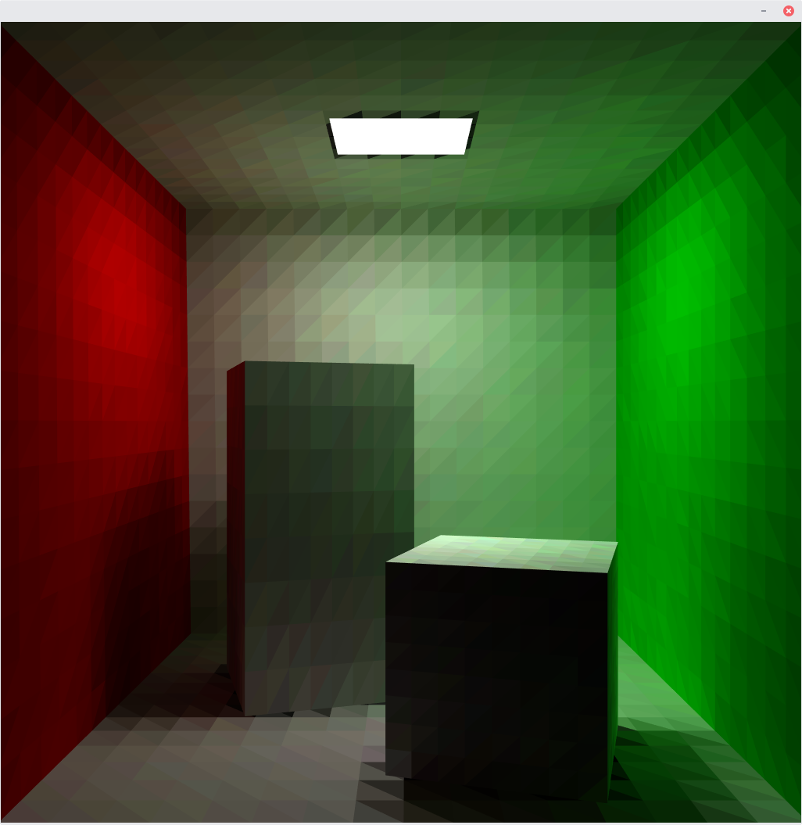
\includegraphics[scale=0.3]{bad_colors.png}
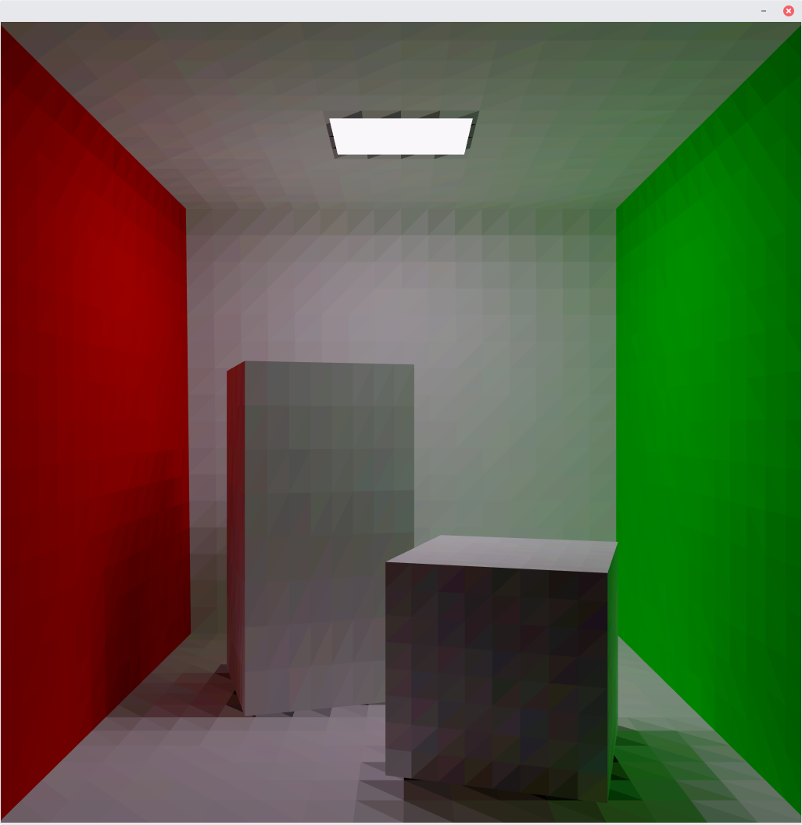
\includegraphics[scale=0.3]{good_colors.png}
\caption*{Рисунок 9 --- Результат применения гамма-коррекции и оператора тональной компрессии}
\end{figure}

\subsection{Отображение результатов}
Последним этапом работы программы полученные в результате работы ИСИМЯ цветовые значения приводились в формат, необоходимый для работы OpenGL API, так как в процессе расчетов испольовался вектор структур типа \texttt{patch}, описанный в листинге 7, а для OpenGL принимает на вход массив значений с плавающей запятой. Необходимые преобразования проводились при помощи функции \texttt{glify}, принимающей вектор структур типа \texttt{patch} и возвращающей вектор значений \texttt{float}, непосредственно пригодный к отрисовке средствами OpenGL. Так как в программе был предусмотрен предпросмотр полигональной модели до окончания расчетов, в функцию также передавался флаг, в зависимости от которого значения цвета могли игнорироваться и полагаться равными некоторой константе:
\begin{lstlisting}
for (const auto p : primitives) {
    vertices.push_back(p->vertices[0].x);
    vertices.push_back(p->vertices[0].y);
    vertices.push_back(p->vertices[0].z);
    vertices.push_back(fill ? 0.6f : p->colors[0].r);
    vertices.push_back(fill ? 0.6f : p->colors[0].g);
    vertices.push_back(fill ? 0.6f : p->colors[0].b);
    ...
}
return vertices;
\end{lstlisting}
\begin{center}Листинг 14 --- Подготовка данных к отрисовке \end{center}

Для демонстрационных целей были также написаны функция \texttt{save\_results}, сохраняющая вектор, возвращенный функцией \texttt{glify} в бинарный файл, и функция \texttt{load\_results}, загружающая готовые данные.

Так как в ходе работы алгоритма цвета отображаемой полигональной модели как минимум один раз изменяются (по окончанию работы алгоритма), для обновления данных была написана функция \texttt{update\_buffers}, использующая метод \texttt{glBufferSubData} OpenGL API. Этот метод вызывался из основного цикла GLFW в случае, если установлен в истинное значение атомарный флаг \texttt{finished\_radiosity}.
\newpage\section{Тестирование}
Тестирование написанной реализации производилось по двум критериям: производительность и качество конечного изображения. Оценка производительности служит лишь проверкой заявленной ассимптотики, так как целью настоящей курсовой работы не являлось написание крайне высокопризводительного приложения. Оценка качества полученных изображений представлена в сравнении с изображением \cite{karlIMG}, полученным при помощи алгоритма двунаправленной трассировки путей.
\subsection{Оценка производительности}
Для оценки производительности была введена функция хрометража, замеряющая время работы всех существенных блоков работы приложения: инициализации, загрузки и обработки полигональной модели, построения BVH-дерева, метода излучательности (в том числе среднее время обработки одного луча) и оператора тональной компрессии.

Время инициализации программы оказалось несущественным, а загрузка модели и построение иерархии ожидаемо показали линейную зависимость от количества полигонов. Более интересной оказалась зависимость время работы метода излучательности от количества полигонов:  логирифмитеская сложность пересечения луча с BVH-деревом привела к тому, что при фиксированном количестве лучей время работы алгоритма росло гораздо медленнее чем количество полигонов отображаемой модели:

\begin{figure}[h]
\centering
\begin{tikzpicture}
\begin{axis}[ 
    xlabel={кол-во полигонов},
    ylabel={время, сек}
  ]
    \addplot[dotted, mark=*] table {
962  4.48
3842  6.01
15362  10.03
61442  15.51
245762  15.77
};
\end{axis}
\end{tikzpicture}
\caption*{Рисунок 10 --- Время работы алгоритма, количество лучей = 500000}
\end{figure}

Также можно убедиться, что время работы метода излучательности не зависит от количества источников света в сцене, что нехарактерно для алгоритмов глобального освещения. Для проверки данного факта была использована обычная сцена с коробкой Корнелла, однако излучатель, состоящий обычно всего из двух полигонов, был разбит на 128. Как и ожидалось, время работы алгоритма не изменилось, а полученные изображения отличаются не больше, чем два изображения полученных повторным запуском программы с одинаковыми входными данным (имеющиеся отличия обусловлены статистической природой получения решения):

\begin{figure}[h]
\centering
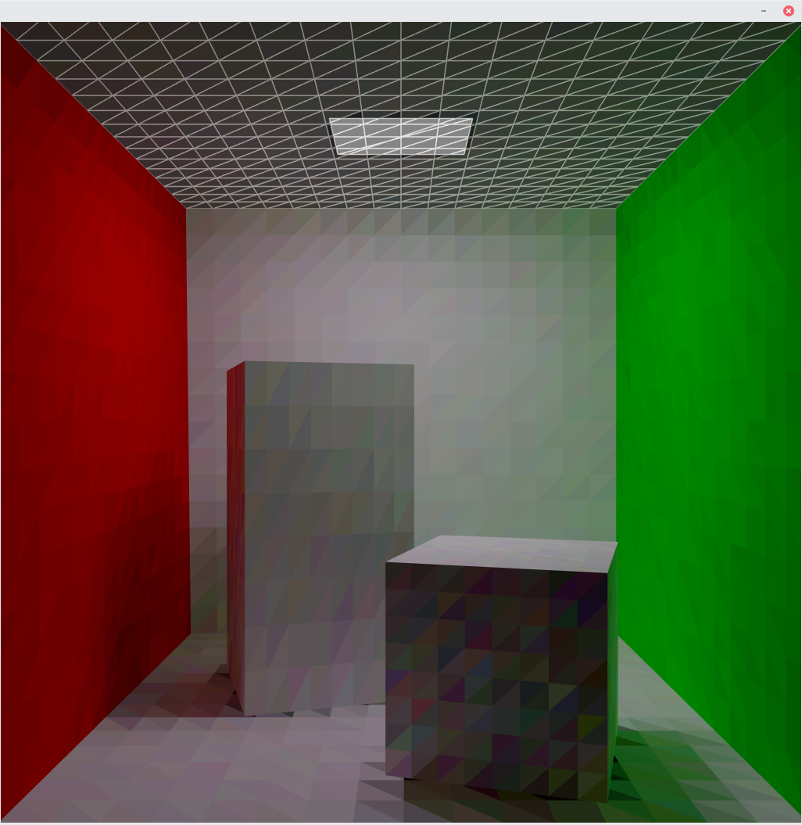
\includegraphics[scale=0.3]{no_tess.png}
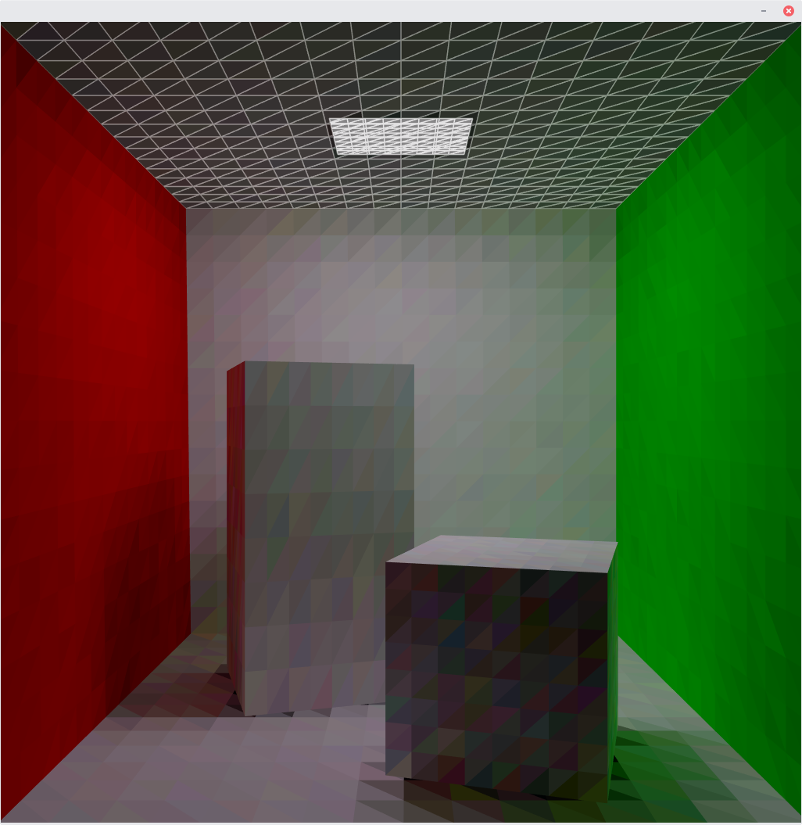
\includegraphics[scale=0.3]{tess.png}
\caption*{Рисунок 10 --- Изменение количества источников света}
\end{figure}

Оба изорбажения, представленные выше, были получены спустя 10 секунд работы алгоритма излучательности. Для сравнения, наивная реализация алгоритма с подсчетом форм-факторов требовала для получения схожего результата приблизительно 30 минут, а на более детализированных моделях (сверх 50000 полигонов) не завершалась сутками!

\subsection{Оценка результатов}
Для оценки достижимого уровня качества изображения была сконструирована полигональная модель с очень высоким уровнем тесселяции (около 250 тысяч полигонов) и запущена симуляция с крайне высоким числом лучей (500 миллионов). С использованием одного потока центрального процессора с тактовой частотой 3.6ГГц расчет занял 173.5 минут, т.е. немного меньше трех часов.

При таком высоком уровне тесселяции необходимость какой-либо интерполяции пропадает, так как участки константой излучательности становятся настолько небольшими, что их практически нельзя различить невооруженным взглядом (со стандартной позиции камеры). По этой причине возможно провести сравнение полученного изображения с полученным при помощи алгоритма двунаправленной трассировки путей \cite{karlIMG} (на рисунке 11 это изображение расположено слева, а полученное в ходе настоящей курсовой работы --- справа).

Сразу же можно заметить, что изображение, полученное трассировкой путей имеет относительно желтоватый окрас. Этот факт объясняется тем, что реализация из \cite{karlIMG} поддерживает входные данные в спектральном формате, которые для модели коробки Корнелла исключительно точно измерены и опубликованы на сайте университета \cite{Cor05}. В том числе при рассмотрении эмиссионного спектра источника света можно заметить, что ``лампа'' в верхней части модели излучает совсем не белый свет.

Вторым заметным отличием являются более выделенные на левом изображении тени в ребрах, смежных с верхней гранью модели. Отсутсвие столь интенсивных теней на правом изображении обусловлено тем, что по определнию метода излучательности излучаемость на каждом участке полагается постоянной, а значит последний ряд участков будет слишком светлым в своей верхней части.

\begin{figure}[h]
\centering
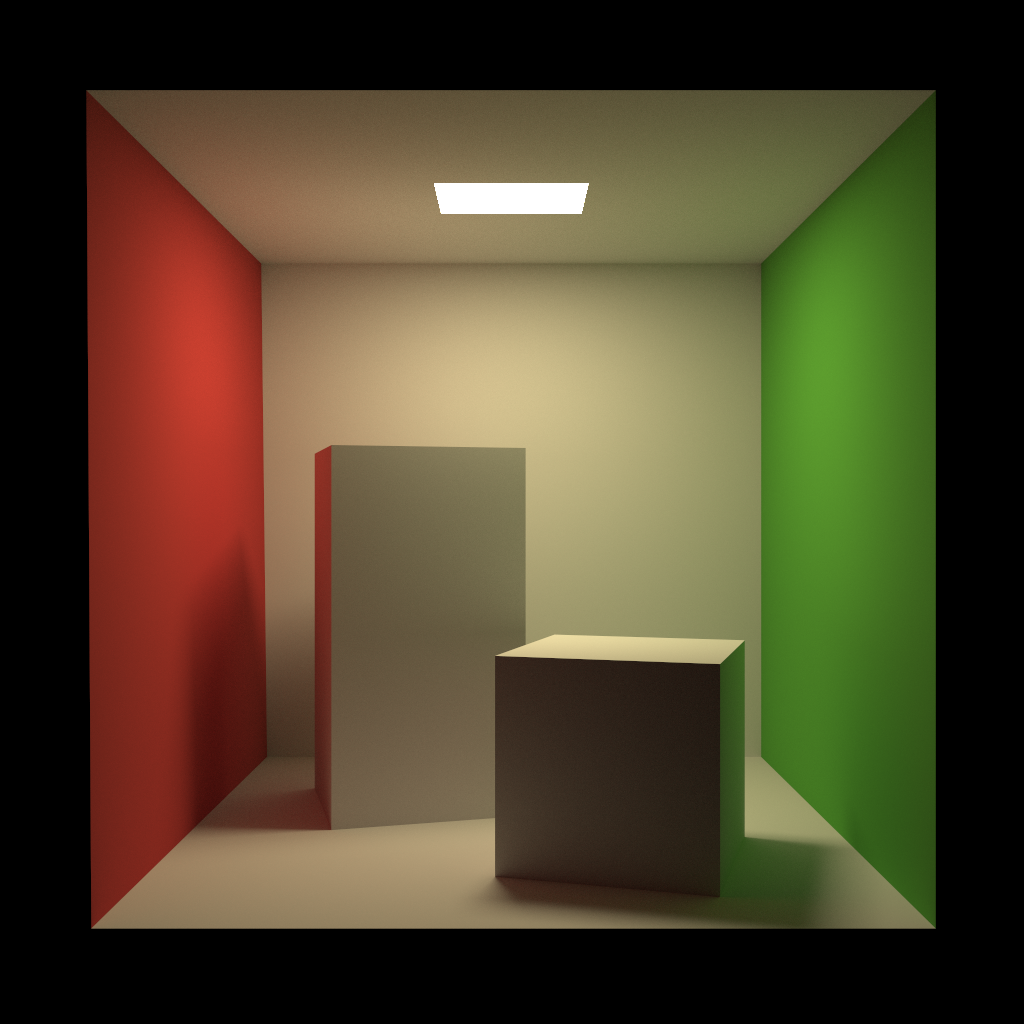
\includegraphics[scale=0.25]{reference_cornell.png}
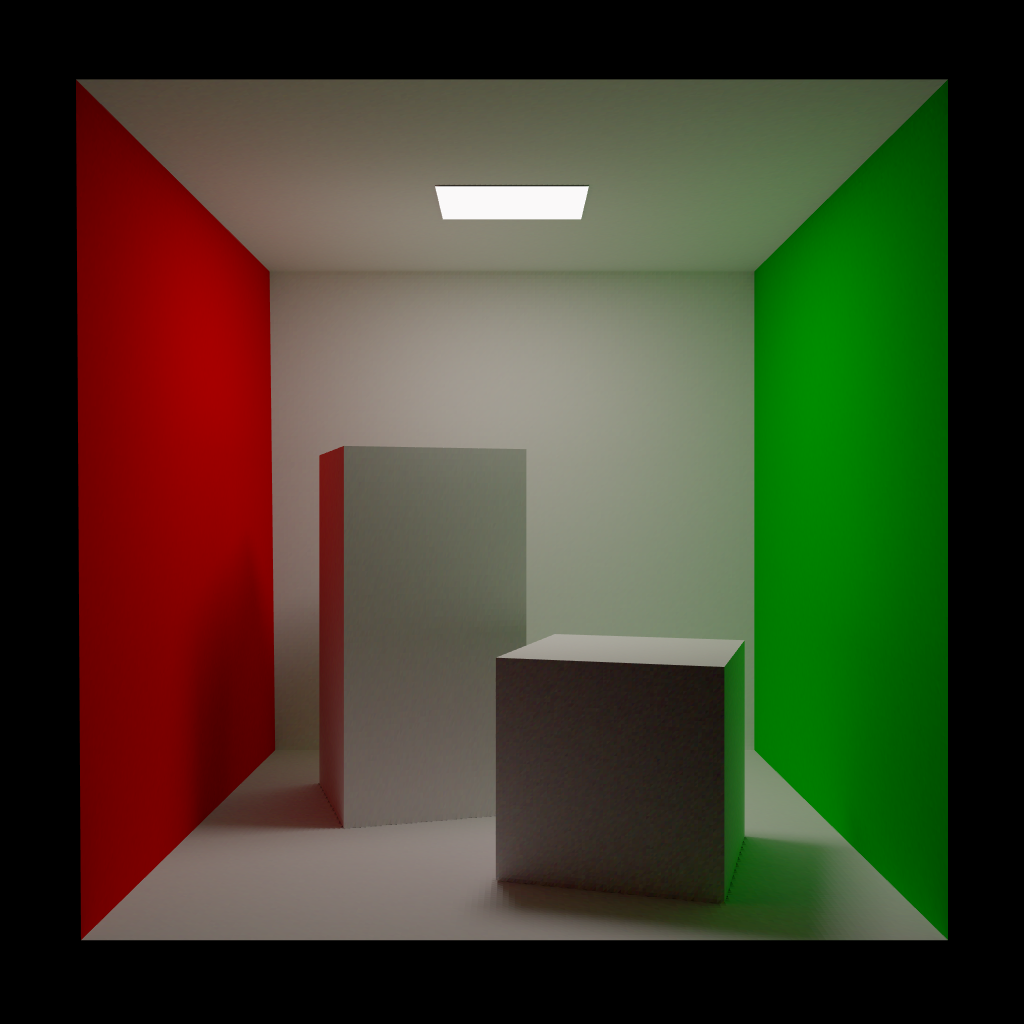
\includegraphics[scale=0.25]{500mil.png}
\caption*{Рисунок 11 --- Результат трехчасовой симуляции, N полигонов = 245762, N лучей = 500000000}
\end{figure}

\newpage\section*{Заключение}
\addcontentsline{toc}{section}{Заключение}

\newpage
\begin{thebibliography}{9} % Источники
\addcontentsline{toc}{section}{Список литературы}
\bibitem{Kaj86} 
Kajiya J.
\textit{The Rendering Equation.} / 
J. Kajiya //
Computer Graphics (SIGGRAPH ’86 Proceedings) --- Dallas, 1986 --- С. 143-150.

\bibitem{Witt80} 
Whitted T.
\textit{An Improved Illumination Model for Shaded Display.} / 
T. Whitted //
Communications of the ACM --- 1980 --- С. 343–349.

\bibitem{Kolb95}
Kolb C.
\textit{A Realistic Camera Model for Computer Graphics.} /
C. Kolb, D. Mitchell, P. Hanrahan //
Computer Graphics (SIGGRAPH ’95 Proceedings) --- Los Angeles, 1995 --- С. 317-324.

\bibitem{karlIMP}
Yining K.
\textit{Importance Sampled Direct Lighting.} / 
K. Yining //
Code and Visuals --- 2013 --- Режим доступа: http://blog.yiningkarlli.com/2013/04/importance-sampled-direct-lighting.html (дата обращения 11.01.2018)

\bibitem{karlBDPT}
Yining K.
\textit{Bidirectional Pathtracing Integrator.} / 
K. Yining //
Code and Visuals --- 2015 --- Режим доступа: http://blog.yiningkarlli.com/2015/02/bidirectional-pathtracing-integrator.html (дата обращения 11.01.2018)

\bibitem{Gor84}
Goral C.
\textit{Modeling the Interaction of Light Between Diffuse Surfaces.} /
C. Goral, K. Torrance, D. Greenberg, B. Battaile //
Computer Graphics (SIGGRAPH ’84 Proceedings) --- Minneapolis, 1984 --- С. 213-222.

\bibitem{Coh93}
Cohen M.
\textit{Radiosity and Realistic Image Synthesis} /Shir90
M. Cohen, J. Wallace
--- Boston: Academic Press Professional, 1993 --- 381 с.

\bibitem{Sch93}
Schr{\"o}der P.
\textit{A closed form expression for the form factor between two polygons} /
P. Schr{\"o}der, P. Hanrahan //
Tech. Rep. CS-404-93 --- Department of Computer Science, Princeton University, 1993.

\bibitem{Pet06}
Peters A.
\textit{Advanced Global Illumination, Second Edition} /
A. Peters, P. Dutre, K. Bala
--- Wellesley, Massachusetts: A K Peters Ltd/CRC Press, 2006 --- 384 c.

\bibitem{Coh85}
Cohen M.
\textit{The Hemi-Cube, A Radiosity Solution for Complex Environments} /
M. Cohen, D. Greenberg //
Computer Graphics (SIGGRAPH ’85 Proceedings) --- San Francisco, 1985 --- С. 31-40.

\bibitem{Shir90}
Shirley P.
\textit{A Ray Tracing Method for Illumination Calculation in Diffuse–Specular Scenes.} /
P.Shirley //
Graphics Interface '90 --- 1990 --- С. 205–212.
1990.

\bibitem{Bek99}
Bekaert P.
\textit{Hierarchical and stochastic algorithms for radiosity} /
P. Bekaert //
Ph.D Thesis --- Department of Computer Science, KU Leuven, Celestijnenlaan 200A, 3001 Heverlee, 1999 --- 276 с.

\bibitem{Kel96}
Keller  A.
\textit{Quasi-Monte Carlo Radiosity.} /
A. Keller //
Eurographics Rendering --- Workshop 1996 --- С. 101–110.

\bibitem{Fuj12}
Fujita S.
\textit{Tiny but powerful single file wavefront obj loader} /
S. Fujita //
GitHub --- 2012 --- Режим доступа: https://github.com/syoyo/tinyobjloader (дата обращения 11.01.2018)

\bibitem{KK86}
Kay T.
\textit{Ray tracing complex scenes.} /
T. Kay, J. Kajiya //
Computer Graphics (SIGGRAPH ’86 Proceedings) --- Dallas, 1986 --- С. 269-278.

\bibitem{Pha17}
Pharr M.
\textit{Physically Based Rendering: From Theory to Implementation. Third Edition.} /
M. Pharr, W. Jakob, G. Humphreys --- Cambridge, 2017 --- 1225 с.

\bibitem{Rei02}
Reinhard E.
\textit{Photographic tone reproduction for digital images.} /
E. Reinhard //
ACM Transactions on Graphics --- 2002 --- С. 21

\bibitem{karlIMG}
Yining K.
\textit{Takua Render Revision 5.} / 
K. Yining //
Code and Visuals --- 2014 --- Режим доступа: https://blog.yiningkarlli.com/2014/12/takua-revision-5.html (дата обращения 11.01.2018)

\bibitem{Cor05}
\textit{Scene Data.} /
Cornell University Program of Computer Graphics //
Cornell Box Data --- 2005 --- Режим доступа: https://www.graphics.cornell.edu/online/box/data.html (дата обращения 11.01.2018)

\end{thebibliography}
\newpage
Термины:

\begin{itemize}
\item[] 'radiosity' --- метод излучательности
\item[] 'radiance' --- энергетическая яркость
\item[] 'importance sampling' --- выборка по значимости
\item[] 'tone mapping' --- тональное отображение / тональная компрессия
\item[] 'sample' --- выборка
\item[] 'cosine distribution' --- распределение косинусов
\item[] 'estimator' --- статистическая оценка
\item[] 'statified sampling' --- районированная выборка
\item[] 'variance reduction' --- методы понижения дисперсии
\item[] 'control variates' --- метод выделения главной части
\end{itemize}
\end{document}